\documentclass[journal=jctc,manuscript=article]{achemso}
\setkeys{acs}{articletitle = true}
 
%%%%%%%%%%%%%%%%%%%%%%%%%%%%%%%%%%%%%%%%%%%%%%%%%%%%%%%%%%%%%%%%%%%%%
%% Place any additional packages needed here.  Only include packages
%% which are essential, to avoid problems later.
%%%%%%%%%%%%%%%%%%%%%%%%%%%%%%%%%%%%%%%%%%%%%%%%%%%%%%%%%%%%%%%%%%%%%
\usepackage{chemformula} % Formula subscripts using \ch{}
\usepackage[T1]{fontenc} % Use modern font encodings

%%%%%%%%%%%%%%%%%%%%%%%%%%%%%%%%%%%%%%%%%%%%%%%%%%%%%%%%%%%%%%%%%%%%%
%% If issues arise when submitting your manuscript, you may want to
%% un-comment the next line.  This provides information on the
%% version of every file you have used.
%%%%%%%%%%%%%%%%%%%%%%%%%%%%%%%%%%%%%%%%%%%%%%%%%%%%%%%%%%%%%%%%%%%%%
%%\listfiles

%%%%%%%%%%%%%%%%%%%%%%%%%%%%%%%%%%%%%%%%%%%%%%%%%%%%%%%%%%%%%%%%%%%%%
%% Place any additional macros here.  Please use \newcommand* where
%% possible, and avoid layout-changing macros (which are not used
%% when typesetting).
%%%%%%%%%%%%%%%%%%%%%%%%%%%%%%%%%%%%%%%%%%%%%%%%%%%%%%%%%%%%%%%%%%%%%
% \newcommand*\mycommand[1]{\texttt{\emph{#1}}}

\usepackage{fullpage}
\usepackage{amsfonts}
\usepackage{graphicx}
\usepackage{float}
\usepackage{amsmath}
\usepackage{chemfig}
\usepackage{indentfirst}
\usepackage{longtable}
\usepackage{array}
\usepackage{cellspace}
\usepackage{palatino}
%\usepackage{breqn}
\usepackage{amssymb}
\usepackage{verbatim}
\usepackage[hidelinks,colorlinks=false,citecolor=black,linkcolor=black]{hyperref}
\usepackage{siunitx}
\usepackage{xr}
%\usepackage{bibentry}
\usepackage{verbatim}

%\DefineVerbatimEnvironment%
%	{verbatimprog}%
%	{Verbatim}%
%	{fontsize=\footnotesize}%

\newenvironment{myequation}{%
\addtocounter{equation}{-1}
\refstepcounter{defcounter}
\renewcommand\theequation{SI.\thedefcounter}
\begin{equation*}}
{\end{equation*}}

\renewcommand{\thefigure}{SI.\arabic{figure}}

\renewcommand{\thepage}{SI.\arabic{page}}

\renewcommand{\thesection}{SI.\Roman{section}}

\renewcommand{\thetable}{SI.\Roman{table}}

\makeatletter
\newcommand*{\addFileDependency}[1]{% argument=file name and extension
	\typeout{(#1)}
	\@addtofilelist{#1}
	\IfFileExists{#1}{}{\typeout{No file #1.}}
}
\makeatother

\newcommand*{\myexternaldocument}[1]{%
	\externaldocument{#1}%
	\addFileDependency{#1.tex}%
	\addFileDependency{#1.aux}%
}

\myexternaldocument{JCED_FOMMS_manuscript}

\SectionNumbersOn

% The figures are in a figures/ subdirectory.
\graphicspath{{figures/}}

%\bibliographystyle{apsrevlong}
%\bibliographystyle{apsrev}
\bibliographystyle{unsrt}
%\bibliographystyle{acs}

% italicized boldface for math (e.g. vectors)
\newcommand{\bfv}[1]{{\mbox{\boldmath{$#1$}}}}
% non-italicized boldface for math (e.g. matrices)
\newcommand{\bfm}[1]{{\bf #1}}          

%\newcommand{\bfm}[1]{{\mbox{\boldmath{$#1$}}}}
%\newcommand{\bfm}[1]{{\bf #1}}
\newcommand{\expect}[1]{\left \langle #1 \right \rangle} % <.> for denoting expectations over realizations of an experiment or thermal averages

\newcommand{\var}[1]{{\mathrm var}{(#1)}}
\newcommand{\x}{\bfv{x}}
\newcommand{\y}{\bfv{y}}
\newcommand{\f}{\bfv{f}}

\newcommand{\hatf}{\hat{f}}

\newcommand{\bTheta}{\bfm{\Theta}}
\newcommand{\btheta}{\bfm{\theta}}
\newcommand{\bhatf}{\bfm{\hat{f}}}
\newcommand{\Cov}[1] {\mathrm{cov}\left( #1 \right)}
\newcommand{\T}{\mathrm{T}}                                % T used in matrix transpose

\author{Richard A. Messerly}
\email{richard.messerly@nist.gov}
\affiliation{Thermodynamics Research Center, National Institute of Standards and Technology, Boulder, Colorado, 80305, United States}

\author{Mohammad S. Barhaghi}
\affiliation{Department of Chemical Engineering and Materials Science, Wayne State University, Detroit, Michigan 48202, United States}

\author{Jeffrey J. Potoff}
\affiliation{Department of Chemical Engineering and Materials Science, Wayne State University, Detroit, Michigan 48202, United States}

\author{Michael R. Shirts}
\affiliation{Department of Chemical and Biological Engineering, University of Colorado, Boulder, Colorado, 80309, United States}

%%%%%%%%%%%%%%%%%%%%%%%%%%%%%%%%%%%%%%%%%%%%%%%%%%%%%%%%%%%%%%%%%%%%%
%% The document title should be given as usual. Some journals require
%% a running title from the author: this should be supplied as an
%% optional argument to \title.
%%%%%%%%%%%%%%%%%%%%%%%%%%%%%%%%%%%%%%%%%%%%%%%%%%%%%%%%%%%%%%%%%%%%%
%\title{Multistate Bennett Acceptance Ratio replaces histogram reweighting for vapor-liquid coexistence calculations}
%\title{Multistate Bennett Acceptance Ratio to enable rapid force field parameterization}
%\title{Multistate Bennett Acceptance Ratio as a substitute for histogram reweighting when optimizing non-bonded parameters}
%\title{Multistate reweighting provides a better alternative to histogram reweighting for coexistance calculations}
%\title{Multistate histogram-free reweighting for vapor-liquid coexistence calculations of non-simulated force field parameters}
%\title{Estimating vapor-liquid coexistence properties with histogram-free reweighting}
%\title{Histogram-free reweighting for vapor-liquid coexistence calculations of multiple force fields}
\title{Supporting information: Histogram-free reweighting to estimate vapor-liquid coexistence properties of non-simulated force fields}

%%%%%%%%%%%%%%%%%%%%%%%%%%%%%%%%%%%%%%%%%%%%%%%%%%%%%%%%%%%%%%%%%%%%%
%% Some journals require a list of abbreviations or keywords to be
%% supplied. These should be set up here, and will be printed after
%% the title and author information, if needed.
%%%%%%%%%%%%%%%%%%%%%%%%%%%%%%%%%%%%%%%%%%%%%%%%%%%%%%%%%%%%%%%%%%%%%
%\abbreviations{IR,NMR,UV}
\keywords{MBAR, Monte Carlo, Grand Canonical, Vapor-liquid equilibria}

%%%%%%%%%%%%%%%%%%%%%%%%%%%%%%%%%%%%%%%%%%%%%%%%%%%%%%%%%%%%%%%%%%%%%
%% The manuscript does not need to include \maketitle, which is
%% executed automatically.
%%%%%%%%%%%%%%%%%%%%%%%%%%%%%%%%%%%%%%%%%%%%%%%%%%%%%%%%%%%%%%%%%%%%%
\begin{document}

\section{State Points} \label{SI sec: State Points}

\begin{table}[htb!]
	\caption{State points simulated for 2-methylpropane with the TraPPE force field.}
	\begin{center}
		\begin{tabular}{|c|c|c|}
			\hline
			$T$ (K) & $\mu$ (K) & $L$ (nm) \\ \hline
			350	&	-3120	&	3.0	\\
			380	&	-3120	&	3.0	\\
			405	&	-3117	&	3.0	\\
			380	&	-2980	&	3.0	\\
			350	&	-2880	&	3.0	\\
			320	&	-2790	&	3.0	\\
			290	&	-2705	&	3.0	\\
			260	&	-2645	&	3.0	\\
			230	&	-2600	&	3.0	\\
			200	&	-2570	&	3.0	\\
			\hline
		\end{tabular}
	\end{center}
\end{table}

\begin{table}[htb!]
	\caption{State points simulated for 2,2-dimethylpropane with the TraPPE force field.}
	\begin{center}
		\begin{tabular}{|c|c|c|}
			\hline
			$T$ (K) & $\mu$ (K) & $L$ (nm) \\ \hline
			380	&	-3405	&	3.0	\\
			410	&	-3405	&	3.0	\\
			440	&	-3405	&	3.0	\\
			410	&	-3250	&	3.0	\\
			380	&	-3140	&	3.0	\\
			350	&	-3037	&	3.0	\\
			330	&	-2970	&	3.0	\\
			300	&	-2900	&	3.0	\\
			270	&	-2820	&	3.0	\\
			\hline
		\end{tabular}
	\end{center}
\end{table}

\begin{table}[htb!]
	\caption{State points simulated for 2,2-dimethylbutane with the TraPPE force field.}
	\begin{center}
		\begin{tabular}{|c|c|c|}
			\hline
			$T$ (K) & $\mu$ (K) & $L$ (nm) \\ \hline
			420	&	-3860	&	3.5	\\
			450	&	-3860	&	3.5	\\
			480	&	-3860	&	3.5	\\
			450	&	-3719	&	3.5	\\
			420	&	-3600	&	3.5	\\
			400	&	-3524	&	3.5	\\
			380	&	-3450	&	3.5	\\
			360	&	-3368	&	3.5	\\
			340	&	-3288	&	3.5	\\
			310	&	-3280	&	3.5	\\
			\hline
		\end{tabular}
	\end{center}
\end{table}

\begin{table}[htb!]
	\caption{State points simulated for 2,3-dimethylbutane with the TraPPE force field.}
	\begin{center}
		\begin{tabular}{|c|c|c|}
			\hline
			$T$ (K) & $\mu$ (K) & $L$ (nm) \\ \hline
			440	&	-4015	&	3.0	\\
			470	&	-4015	&	3.0	\\
			500	&	-4011	&	3.0	\\
			470	&	-3845	&	3.0	\\
			440	&	-3735	&	3.0	\\
			410	&	-3635	&	3.0	\\
			380	&	-3555	&	3.0	\\
			350	&	-3480	&	3.0	\\
			320	&	-3415	&	3.0	\\
			\hline
		\end{tabular}
	\end{center}
\end{table}

\begin{table}[htb!]
	\caption{State points simulated for 3,3-dimethylhexane with the TraPPE force field.}
	\begin{center}
		\begin{tabular}{|c|c|c|}
			\hline
			$T$ (K) & $\mu$ (K) & $L$ (nm) \\ \hline
			500	&	-4670	&	3.5	\\
			530	&	-4670	&	3.5	\\
			560	&	-4670	&	3.5	\\
			520	&	-4476	&	3.5	\\
			490	&	-4370	&	3.5	\\
			460	&	-4268	&	3.5	\\
			430	&	-4164	&	3.5	\\
			400	&	-4039	&	3.5	\\
			370	&	-3925	&	3.5	\\
			\hline
		\end{tabular}
	\end{center}
\end{table}

\begin{table}[htb!]
	\caption{State points simulated for 3-methyl-3-ethylpentane with the TraPPE force field.}
	\begin{center}
		\begin{tabular}{|c|c|c|}
			\hline
			$T$ (K) & $\mu$ (K) & $L$ (nm) \\ \hline
			500	&	-4785	&	4.0	\\
			550	&	-4785	&	4.0	\\
			580	&	-4785	&	4.0	\\
			550	&	-4636	&	4.0	\\
			520	&	-4520	&	4.0	\\
			490	&	-4400	&	4.0	\\
			460	&	-4280	&	4.0	\\
			430	&	-4160	&	4.0	\\
			410	&	-4080	&	4.0	\\
			390	&	-3990	&	4.0	\\
			\hline
		\end{tabular}
	\end{center}
\end{table}

\begin{table}[htb!]
	\caption{State points simulated for 2,3,4-trimethylpentane with the TraPPE force field.}
	\begin{center}
		\begin{tabular}{|c|c|c|}
			\hline
			$T$ (K) & $\mu$ (K) & $L$ (nm) \\ \hline
			480	&	-4740	&	3.5	\\
			520	&	-4740	&	3.5	\\
			565	&	-4735	&	3.5	\\
			530	&	-4549	&	3.5	\\
			500	&	-4436	&	3.5	\\
			470	&	-4337	&	3.5	\\
			440	&	-4241	&	3.5	\\
			410	&	-4182	&	3.5	\\
			380	&	-4090	&	3.5	\\
			350	&	-4020	&	3.5	\\
			\hline
		\end{tabular}
	\end{center}
\end{table}

\begin{table}[htb!]
	\caption{State points simulated for 2,2,4-trimethylpentane with the TraPPE force field.}
	\begin{center}
		\begin{tabular}{|c|c|c|}
			\hline
			$T$ (K) & $\mu$ (K) & $L$ (nm) \\ \hline
			480	&	-4600	&	4.0	\\
			530	&	-4600	&	4.0	\\
			560	&	-4600	&	4.0	\\
			530	&	-4450	&	4.0	\\
			500	&	-4330	&	4.0	\\
			470	&	-4210	&	4.0	\\
			440	&	-4090	&	4.0	\\
			410	&	-3960	&	4.0	\\
			380	&	-3840	&	4.0	\\
			\hline
		\end{tabular}
	\end{center}
\end{table}

\begin{table}[htb!]
	\caption{State points simulated for cyclohexane with the TraPPE force field.}
	\begin{center}
		\begin{tabular}{|c|c|c|}
			\hline
			$T$ (K) & $\mu$ (K) & $L$ (nm) \\ \hline
			450	&	-4350	&	3.0	\\
			500	&	-4350	&	3.0	\\
			550	&	-4350	&	3.0	\\
			500	&	-4120	&	3.0	\\
			460	&	-3977	&	3.0	\\
			410	&	-3790	&	3.0	\\
			350	&	-3562	&	3.0	\\
			\hline
		\end{tabular}
	\end{center}
\end{table}

\begin{table}[htb!]
	\caption{State points simulated for cyclohexane with the $\lambda^{(1)}_{\rm CH_2} = 14$ force field.}
	\begin{center}
		\begin{tabular}{|c|c|c|}
			\hline
			$T$ (K) & $\mu$ (K) & $L$ (nm) \\ \hline
			450	&	-4389	&	3.0	\\
			500	&	-4389	&	3.0	\\
			550	&	-4389	&	3.0	\\
			500	&	-4164	&	3.0	\\
			460	&	-4033	&	3.0	\\
			410	&	-3891	&	3.0	\\
			360	&	-3780	&	3.0	\\
			\hline
		\end{tabular}
	\end{center}
\end{table}

\begin{table}[htb!]
	\caption{State points simulated for cyclohexane with the $\lambda^{(1)}_{\rm CH_2} = 16$ force field.}
	\begin{center}
		\begin{tabular}{|c|c|c|}
			\hline
			$T$ (K) & $\mu$ (K) & $L$ (nm) \\ \hline
			450	&	-4367	&	3.0	\\
			500	&	-4367	&	3.0	\\
			550	&	-4367	&	3.0	\\
			500	&	-4149	&	3.0	\\
			460	&	-4024	&	3.0	\\
			410	&	-3893	&	3.0	\\
			360	&	-3792	&	3.0	\\
			\hline
		\end{tabular}
	\end{center}
\end{table}

\begin{table}[htb!]
	\caption{State points simulated for cyclohexane with the $\lambda^{(1)}_{\rm CH_2} = 18$ force field.}
	\begin{center}
		\begin{tabular}{|c|c|c|}
			\hline
			$T$ (K) & $\mu$ (K) & $L$ (nm) \\ \hline
			450	&	-4370	&	3.0	\\
			500	&	-4370	&	3.0	\\
			550	&	-4370	&	3.0	\\
			500	&	-4158	&	3.0	\\
			460	&	-4037	&	3.0	\\
			410	&	-3912	&	3.0	\\
			360	&	-3825	&	3.0	\\
			\hline
		\end{tabular}
	\end{center}
\end{table}

\begin{table}[htb!]
	\caption{State points simulated for cyclohexane with the $\lambda^{(1)}_{\rm CH_2} = 20$ force field.}
	\begin{center}
		\begin{tabular}{|c|c|c|}
			\hline
			$T$ (K) & $\mu$ (K) & $L$ (nm) \\ \hline
			450	&	-4386	&	3.0	\\
			500	&	-4386	&	3.0	\\
			550	&	-4386	&	3.0	\\
			500	&	-4178	&	3.0	\\
			460	&	-4062	&	3.0	\\
			410	&	-3946	&	3.0	\\
			360	&	-3866	&	3.0	\\
			\hline
		\end{tabular}
	\end{center}
\end{table}

\begin{table}[htb!]
	\caption{State points simulated for 2-methylpropane with the MiPPE-gen force field.}
	\begin{center}
		\begin{tabular}{|c|c|c|}
			\hline
			$T$ (K) & $\mu$ (K) & $L$ (nm) \\ \hline
            350	&	-3150	&	3.0	\\
            380	&	-3150	&	3.0	\\
            410	&	-3145	&	3.0	\\
            380	&	-3010	&	3.0	\\
            350	&	-2910	&	3.0	\\
            320	&	-2830	&	3.0	\\
            290	&	-2760	&	3.0	\\
            260	&	-2700	&	3.0	\\
            230	&	-2670	&	3.0	\\
            200	&	-2640	&	3.0	\\
            \hline
		\end{tabular}
	\end{center}
\end{table}

\begin{table}[htb!]
	\caption{State points simulated for 2,2-dimethylpropane with the MiPPE-gen force field.}
	\begin{center}
		\begin{tabular}{|c|c|c|}
			\hline
			$T$ (K) & $\mu$ (K) & $L$ (nm) \\ \hline
			368	&	-3344	&	3.0	\\
			398	&	-3344	&	3.0	\\
			430	&	-3400	&	3.0	\\
			398	&	-3216	&	3.0	\\
			372	&	-3124	&	3.0	\\
			346	&	-3032	&	3.0	\\
			326	&	-2961	&	3.0	\\
			299	&	-2865	&	3.0	\\
			270	&	-2759	&	3.0	\\
			\hline
		\end{tabular}
	\end{center}
\end{table}

\begin{table}[htb!]
	\caption{State points simulated for 2,2-dimethylbutane with the MiPPE-gen force field.}
	\begin{center}
		\begin{tabular}{|c|c|c|}
			\hline
			$T$ (K) & $\mu$ (K) & $L$ (nm) \\ \hline
			415	&	-3873	&	3.5	\\
			445	&	-3873	&	3.5	\\
			480	&	-3895	&	3.5	\\
			450	&	-3756	&	3.5	\\
			420	&	-3654	&	3.5	\\
			400	&	-3588	&	3.5	\\
			380	&	-3521	&	3.5	\\
			360	&	-3454	&	3.5	\\
			340	&	-3384	&	3.5	\\
			310	&	-3380	&	3.5	\\
			\hline
		\end{tabular}
	\end{center}
\end{table}

\begin{table}[htb!]
	\caption{State points simulated for 2,3-dimethylbutane with the MiPPE-gen force field.}
	\begin{center}
		\begin{tabular}{|c|c|c|}
			\hline
			$T$ (K) & $\mu$ (K) & $L$ (nm) \\ \hline
			440	&	-4010	&	3.0	\\
			470	&	-4010	&	3.0	\\
			500	&	-4009	&	3.0	\\
			470	&	-3860	&	3.0	\\
			440	&	-3760	&	3.0	\\
			410	&	-3670	&	3.0	\\
			380	&	-3600	&	3.0	\\
			350	&	-3530	&	3.0	\\
			320	&	-3480	&	3.0	\\
			\hline
		\end{tabular}
	\end{center}
\end{table}

\begin{table}[htb!]
	\caption{State points simulated for 2,3,4-trimethylpentane with the MiPPE-gen force field.}
	\begin{center}
		\begin{tabular}{|c|c|c|}
			\hline
			$T$ (K) & $\mu$ (K) & $L$ (nm) \\ \hline
			480	&	-4720	&	3.5	\\
			520	&	-4720	&	3.5	\\
			565	&	-4713	&	3.5	\\
			530	&	-4540	&	3.5	\\
			500	&	-4360	&	3.5	\\
			470	&	-4355	&	3.5	\\
			440	&	-4275	&	3.5	\\
			410	&	-4205	&	3.5	\\
			380	&	-4165	&	3.5	\\
			350	&	-4115	&	3.5	\\
			\hline
		\end{tabular}
	\end{center}
\end{table}

\begin{table}[htb!]
	\caption{State points simulated for 2,2,4-trimethylpentane with the MiPPE-gen force field.}
	\begin{center}
		\begin{tabular}{|c|c|c|}
			\hline
			$T$ (K) & $\mu$ (K) & $L$ (nm) \\ \hline
			470	&	-4570	&	4.0	\\
			520	&	-4570	&	4.0	\\
			550	&	-4570	&	4.0	\\
			520	&	-4420	&	4.0	\\
			490	&	-4300	&	4.0	\\
			460	&	-4170	&	4.0	\\
			430	&	-4050	&	4.0	\\
			400	&	-3920	&	4.0	\\
			370	&	-3790	&	4.0	\\
			\hline
		\end{tabular}
	\end{center}
\end{table}

\section{Tabulated GCMC-MBAR results} \label{SI sec: Tabulated MBAR results}

\subsection{Cyclohexane}

\subsection{Branched alkanes}

\begin{table}[htb!]
	\caption{GCMC-MBAR results for 2-methylpentane with the MiPPE-SL force field. Subscripts correspond to the 95\% confidence interval computed with bootstrap re-sampling.}
	\begin{center}
		\begin{tabular}{|c|c|c|c|c|c|}
			\hline
			$T^{\rm sat}$ (K) & $\rho_{\rm liq}^{\rm sat}$ (kg/m$^3$) & $\rho_{\rm vap}^{\rm sat}$ (kg/m$^3$) & $P_{\rm vap}^{\rm sat}$ (MPa) & $\Delta H_{\rm v}$ (kJ/mol) & $Z_{\rm vap}^{\rm sat}$ \\ \hline
			470 & $422.20_{0.56}$ & $76.7_{1.5}$ & $20.68_{0.17}$ & $14.14_{0.11}$ & $0.595_{0.012}$ \\
			460 & $444.71_{0.79}$ & $61.2_{1.2}$ & $17.61_{0.13}$ & $16.06_{0.12}$ & $0.649_{0.013}$ \\
			450 & $464.38_{0.87}$ & $49.31_{0.88}$ & $14.918_{0.096}$ & $17.71_{0.11}$ & $0.697_{0.013}$ \\
			440 & $481.69_{0.77}$ & $40.17_{0.64}$ & $12.557_{0.068}$ & $19.106_{0.090}$ & $0.736_{0.012}$ \\
			430 & $497.34_{0.70}$ & $32.86_{0.47}$ & $10.491_{0.045}$ & $20.318_{0.074}$ & $0.770_{0.012}$ \\
			420 & $511.89_{0.78}$ & $26.86_{0.36}$ & $8.690_{0.027}$ & $21.408_{0.068}$ & $0.798_{0.011}$ \\
			410 & $525.69_{0.84}$ & $21.87_{0.29}$ & $7.130_{0.017}$ & $22.412_{0.069}$ & $0.824_{0.011}$ \\
			400 & $538.82_{0.88}$ & $17.70_{0.25}$ & $5.788_{0.020}$ & $23.344_{0.069}$ & $0.848_{0.012}$ \\
			390 & $551.23_{0.87}$ & $14.21_{0.22}$ & $4.645_{0.031}$ & $24.207_{0.075}$ & $0.869_{0.014}$ \\
			380 & $562.89_{0.80}$ & $11.30_{0.19}$ & $3.681_{0.042}$ & $25.004_{0.096}$ & $0.888_{0.018}$ \\
			370 & $573.96_{0.88}$ & $8.90_{0.16}$ & $2.878_{0.051}$ & $25.75_{0.14}$ & $0.906_{0.023}$ \\
			360 & $584.8_{1.1}$ & $6.92_{0.14}$ & $2.215_{0.059}$ & $26.46_{0.18}$ & $0.922_{0.031}$ \\
			350 & $595.6_{1.2}$ & $5.31_{0.12}$ & $1.677_{0.065}$ & $27.15_{0.22}$ & $0.935_{0.042}$ \\
			340 & $606.3_{1.2}$ & $4.01_{0.10}$ & $1.245_{0.070}$ & $27.83_{0.27}$ & $0.947_{0.059}$ \\
			330 & $616.4_{1.0}$ & $2.969_{0.085}$ & $0.906_{0.074}$ & $28.45_{0.32}$ & $0.958_{0.083}$ \\
			320 & $625.82_{0.57}$ & $2.156_{0.068}$ & $0.644_{0.078}$ & $29.04_{0.40}$ & $0.97_{0.12}$ \\
			\hline
		\end{tabular}
	\end{center}
\end{table}

\begin{table}[htb!]
	\caption{GCMC-MBAR results for 2-methylhexane with the MiPPE-SL force field. Subscripts correspond to the 95\% confidence interval computed with bootstrap re-sampling.}
	\begin{center}
		\begin{tabular}{|c|c|c|c|c|c|}
			\hline
			$T^{\rm sat}$ (K) & $\rho_{\rm liq}^{\rm sat}$ (kg/m$^3$) & $\rho_{\rm vap}^{\rm sat}$ (kg/m$^3$) & $P_{\rm vap}^{\rm sat}$ (MPa) & $\Delta H_{\rm v}$ (kJ/mol) & $Z_{\rm vap}^{\rm sat}$ \\ \hline
			510 & $406.8_{3.4}$ & $88.4_{2.0}$ & $20.92_{0.11}$ & $14.14_{0.12}$ & $0.559_{0.013}$ \\
			500 & $431.2_{2.2}$ & $70.0_{1.6}$ & $17.989_{0.052}$ & $16.506_{0.085}$ & $0.620_{0.014}$ \\
			490 & $452.1_{1.2}$ & $56.5_{1.0}$ & $15.403_{0.041}$ & $18.472_{0.088}$ & $0.671_{0.013}$ \\
			480 & $470.38_{0.73}$ & $46.30_{0.50}$ & $13.120_{0.056}$ & $20.092_{0.065}$ & $0.7116_{8.3e-3}$ \\
			470 & $486.88_{0.50}$ & $38.21_{0.17}$ & $11.104_{0.062}$ & $21.497_{0.034}$ & $0.7453_{5.3e-3}$ \\
			460 & $502.20_{0.37}$ & $31.56_{0.16}$ & $9.327_{0.058}$ & $22.762_{0.022}$ & $0.7744_{6.2e-3}$ \\
			450 & $516.52_{0.39}$ & $26.01_{0.17}$ & $7.772_{0.050}$ & $23.921_{0.024}$ & $0.8003_{7.3e-3}$ \\
			440 & $530.01_{0.34}$ & $21.34_{0.15}$ & $6.417_{0.043}$ & $24.994_{0.024}$ & $0.8236_{7.9e-3}$ \\
			430 & $542.86_{0.37}$ & $17.41_{0.14}$ & $5.245_{0.039}$ & $25.998_{0.031}$ & $0.8444_{9.1e-3}$ \\
			420 & $554.93_{0.46}$ & $14.10_{0.13}$ & $4.241_{0.037}$ & $26.928_{0.041}$ & $0.863_{0.011}$ \\
			410 & $566.22_{0.43}$ & $11.32_{0.14}$ & $3.390_{0.036}$ & $27.789_{0.046}$ & $0.881_{0.014}$ \\
			400 & $577.21_{0.43}$ & $8.99_{0.14}$ & $2.674_{0.037}$ & $28.610_{0.060}$ & $0.896_{0.019}$ \\
			390 & $588.02_{0.38}$ & $7.06_{0.15}$ & $2.080_{0.039}$ & $29.403_{0.089}$ & $0.910_{0.026}$ \\
			380 & $598.35_{0.22}$ & $5.47_{0.16}$ & $1.593_{0.044}$ & $30.15_{0.14}$ & $0.923_{0.037}$ \\
			370 & $608.04_{0.19}$ & $4.18_{0.16}$ & $1.200_{0.050}$ & $30.85_{0.20}$ & $0.935_{0.053}$ \\
			360 & $617.49_{0.27}$ & $3.14_{0.16}$ & $0.888_{0.057}$ & $31.52_{0.28}$ & $0.945_{0.077}$ \\
			350 & $627.22_{0.26}$ & $2.32_{0.15}$ & $0.644_{0.065}$ & $32.20_{0.39}$ & $0.96_{0.11}$ \\
			\hline
		\end{tabular}
	\end{center}
\end{table}

\begin{table}[htb!]
	\caption{GCMC-MBAR results for 3-methylpentane with the MiPPE-SL force field. Subscripts correspond to the 95\% confidence interval computed with bootstrap re-sampling.}
	\begin{center}
		\begin{tabular}{|c|c|c|c|c|c|}
			\hline
			$T^{\rm sat}$ (K) & $\rho_{\rm liq}^{\rm sat}$ (kg/m$^3$) & $\rho_{\rm vap}^{\rm sat}$ (kg/m$^3$) & $P_{\rm vap}^{\rm sat}$ (MPa) & $\Delta H_{\rm v}$ (kJ/mol) & $Z_{\rm vap}^{\rm sat}$ \\ \hline
			480 & $415.8_{1.5}$ & $84_{24}$ & $23.1_{2.4}$ & $13.7_{1.3}$ & $0.60_{0.18}$ \\
			470 & $440.0_{2.3}$ & $67_{24}$ & $19.9_{1.4}$ & $15.6_{1.7}$ & $0.65_{0.23}$ \\
			460 & $459.8_{2.5}$ & $55_{18}$ & $16.98_{0.59}$ & $17.2_{1.6}$ & $0.69_{0.22}$ \\
			450 & $477.1_{1.9}$ & $45.4_{7.6}$ & $14.43_{0.12}$ & $18.52_{0.94}$ & $0.73_{0.12}$ \\
			440 & $493.2_{1.2}$ & $37.5_{1.5}$ & $12.17_{0.14}$ & $19.74_{0.27}$ & $0.764_{0.032}$ \\
			430 & $508.9_{1.4}$ & $30.95_{0.38}$ & $10.19_{0.15}$ & $20.87_{0.11}$ & $0.794_{0.015}$ \\
			420 & $523.6_{1.1}$ & $25.42_{0.36}$ & $8.45_{0.14}$ & $21.917_{0.094}$ & $0.821_{0.018}$ \\
			410 & $536.8_{1.4}$ & $20.78_{0.32}$ & $6.95_{0.14}$ & $22.85_{0.12}$ & $0.845_{0.021}$ \\
			400 & $548.9_{1.7}$ & $16.89_{0.24}$ & $5.65_{0.13}$ & $23.69_{0.15}$ & $0.867_{0.023}$ \\
			390 & $560.5_{1.5}$ & $13.63_{0.21}$ & $4.55_{0.12}$ & $24.49_{0.13}$ & $0.887_{0.027}$ \\
			380 & $571.8_{1.2}$ & $10.88_{0.20}$ & $3.61_{0.10}$ & $25.250_{0.099}$ & $0.905_{0.031}$ \\
			370 & $582.3_{1.1}$ & $8.59_{0.18}$ & $2.829_{0.089}$ & $25.950_{0.093}$ & $0.922_{0.035}$ \\
			360 & $593.0_{1.1}$ & $6.70_{0.16}$ & $2.185_{0.077}$ & $26.64_{0.12}$ & $0.939_{0.040}$ \\
			350 & $603.8_{1.0}$ & $5.15_{0.14}$ & $1.661_{0.067}$ & $27.33_{0.14}$ & $0.955_{0.047}$ \\
			\hline
		\end{tabular}
	\end{center}
\end{table}

\begin{table}[htb!]
	\caption{GCMC-MBAR results for 3-methylhexane with the MiPPE-SL force field. Subscripts correspond to the 95\% confidence interval computed with bootstrap re-sampling.}
	\begin{center}
		\begin{tabular}{|c|c|c|c|c|c|}
			\hline
			$T^{\rm sat}$ (K) & $\rho_{\rm liq}^{\rm sat}$ (kg/m$^3$) & $\rho_{\rm vap}^{\rm sat}$ (kg/m$^3$) & $P_{\rm vap}^{\rm sat}$ (MPa) & $\Delta H_{\rm v}$ (kJ/mol) & $Z_{\rm vap}^{\rm sat}$ \\ \hline
			520 & $398.4_{4.6}$ & $98.1_{1.2}$ & $23.07_{0.18}$ & $13.25_{0.29}$ & $0.5453_{7.9e-3}$ \\
			510 & $426.2_{3.4}$ & $77.3_{1.3}$ & $19.96_{0.15}$ & $15.86_{0.21}$ & $0.610_{0.011}$ \\
			500 & $449.0_{1.8}$ & $62.6_{1.1}$ & $17.20_{0.12}$ & $17.92_{0.14}$ & $0.662_{0.013}$ \\
			490 & $467.85_{0.87}$ & $51.64_{0.76}$ & $14.74_{0.11}$ & $19.56_{0.10}$ & $0.702_{0.011}$ \\
			480 & $484.12_{0.71}$ & $42.82_{0.51}$ & $12.562_{0.093}$ & $20.963_{0.074}$ & $0.737_{0.010}$ \\
			470 & $498.93_{0.76}$ & $35.54_{0.44}$ & $10.638_{0.075}$ & $22.215_{0.069}$ & $0.768_{0.011}$ \\
			460 & $512.9_{1.0}$ & $29.46_{0.42}$ & $8.944_{0.056}$ & $23.366_{0.088}$ & $0.796_{0.012}$ \\
			450 & $526.2_{1.3}$ & $24.34_{0.36}$ & $7.463_{0.040}$ & $24.442_{0.093}$ & $0.821_{0.013}$ \\
			440 & $539.09_{0.79}$ & $20.03_{0.26}$ & $6.171_{0.029}$ & $25.454_{0.048}$ & $0.844_{0.011}$ \\
			430 & $551.25_{0.90}$ & $16.38_{0.15}$ & $5.055_{0.025}$ & $26.397_{0.089}$ & $0.8648_{8.9e-3}$ \\
			420 & $563.0_{1.6}$ & $13.302_{0.087}$ & $4.097_{0.025}$ & $27.29_{0.16}$ & $0.8838_{7.9e-3}$ \\
			410 & $574.5_{1.4}$ & $10.70_{0.12}$ & $3.283_{0.024}$ & $28.15_{0.18}$ & $0.902_{0.012}$ \\
			400 & $585.3_{1.3}$ & $8.53_{0.18}$ & $2.598_{0.021}$ & $28.96_{0.19}$ & $0.918_{0.021}$ \\
			390 & $595.7_{2.4}$ & $6.72_{0.26}$ & $2.028_{0.021}$ & $29.72_{0.30}$ & $0.933_{0.037}$ \\
			380 & $605.9_{2.8}$ & $5.23_{0.33}$ & $1.560_{0.032}$ & $30.45_{0.41}$ & $0.947_{0.063}$ \\
			370 & $615.4_{1.3}$ & $4.01_{0.38}$ & $1.181_{0.053}$ & $31.13_{0.47}$ & $0.96_{0.10}$ \\
			360 & $624.92_{0.55}$ & $3.04_{0.40}$ & $0.878_{0.081}$ & $31.78_{0.63}$ & $0.97_{0.16}$ \\
			\hline
		\end{tabular}
	\end{center}
\end{table}

\begin{table}[htb!]
	\caption{GCMC-MBAR results for 2,3-dimethylpentane with the MiPPE-SL force field. Subscripts correspond to the 95\% confidence interval computed with bootstrap re-sampling.}
	\begin{center}
		\begin{tabular}{|c|c|c|c|c|c|}
			\hline
			$T^{\rm sat}$ (K) & $\rho_{\rm liq}^{\rm sat}$ (kg/m$^3$) & $\rho_{\rm vap}^{\rm sat}$ (kg/m$^3$) & $P_{\rm vap}^{\rm sat}$ (MPa) & $\Delta H_{\rm v}$ (kJ/mol) & $Z_{\rm vap}^{\rm sat}$ \\ \hline
			510 & $427.9_{1.6}$ & $81_{10}$ & $20.82_{0.91}$ & $15.20_{0.53}$ & $0.606_{0.081}$ \\
			500 & $451.7_{1.0}$ & $66.3_{9.6}$ & $18.00_{0.57}$ & $17.17_{0.70}$ & $0.654_{0.097}$ \\
			490 & $471.41_{0.86}$ & $54.7_{7.1}$ & $15.49_{0.28}$ & $18.83_{0.70}$ & $0.696_{0.091}$ \\
			480 & $488.48_{0.89}$ & $45.5_{4.0}$ & $13.245_{0.092}$ & $20.25_{0.54}$ & $0.731_{0.064}$ \\
			470 & $503.90_{0.73}$ & $37.9_{1.7}$ & $11.257_{0.050}$ & $21.50_{0.32}$ & $0.762_{0.035}$ \\
			460 & $518.28_{0.52}$ & $31.50_{0.62}$ & $9.501_{0.072}$ & $22.64_{0.14}$ & $0.790_{0.017}$ \\
			450 & $532.03_{0.63}$ & $26.12_{0.25}$ & $7.956_{0.080}$ & $23.709_{0.054}$ & $0.816_{0.011}$ \\
			440 & $545.26_{0.62}$ & $21.57_{0.18}$ & $6.606_{0.080}$ & $24.711_{0.037}$ & $0.839_{0.012}$ \\
			430 & $557.77_{0.54}$ & $17.70_{0.16}$ & $5.435_{0.075}$ & $25.646_{0.038}$ & $0.860_{0.014}$ \\
			420 & $569.33_{0.53}$ & $14.43_{0.15}$ & $4.426_{0.070}$ & $26.504_{0.037}$ & $0.880_{0.016}$ \\
			410 & $580.03_{0.59}$ & $11.68_{0.14}$ & $3.565_{0.063}$ & $27.290_{0.040}$ & $0.897_{0.019}$ \\
			400 & $590.33_{0.66}$ & $9.36_{0.13}$ & $2.837_{0.057}$ & $28.032_{0.047}$ & $0.913_{0.022}$ \\
			390 & $600.50_{0.61}$ & $7.43_{0.11}$ & $2.229_{0.052}$ & $28.747_{0.057}$ & $0.927_{0.026}$ \\
			380 & $610.33_{0.59}$ & $5.831_{0.094}$ & $1.726_{0.048}$ & $29.424_{0.079}$ & $0.939_{0.030}$ \\
			370 & $620.01_{0.64}$ & $4.512_{0.077}$ & $1.315_{0.046}$ & $30.08_{0.11}$ & $0.950_{0.037}$ \\
			360 & $630.25_{0.55}$ & $3.438_{0.066}$ & $0.984_{0.045}$ & $30.75_{0.14}$ & $0.959_{0.048}$ \\
			350 & $640.58_{0.49}$ & $2.572_{0.058}$ & $0.722_{0.046}$ & $31.42_{0.20}$ & $0.966_{0.065}$ \\
			\hline
		\end{tabular}
	\end{center}
\end{table}

\begin{table}[htb!]
	\caption{GCMC-MBAR results for 2,3-dimethylhexane with the MiPPE-SL force field. Subscripts correspond to the 95\% confidence interval computed with bootstrap re-sampling.}
	\begin{center}
		\begin{tabular}{|c|c|c|c|c|c|}
			\hline
			$T^{\rm sat}$ (K) & $\rho_{\rm liq}^{\rm sat}$ (kg/m$^3$) & $\rho_{\rm vap}^{\rm sat}$ (kg/m$^3$) & $P_{\rm vap}^{\rm sat}$ (MPa) & $\Delta H_{\rm v}$ (kJ/mol) & $Z_{\rm vap}^{\rm sat}$ \\ \hline
			540 & $422.2_{1.1}$ & $84.5_{3.7}$ & $19.48_{0.48}$ & $15.98_{0.12}$ & $0.586_{0.029}$ \\
			530 & $445.87_{0.82}$ & $68.6_{3.6}$ & $16.89_{0.36}$ & $18.23_{0.22}$ & $0.638_{0.036}$ \\
			520 & $466.30_{0.66}$ & $56.3_{3.0}$ & $14.58_{0.24}$ & $20.17_{0.26}$ & $0.684_{0.038}$ \\
			510 & $484.13_{0.59}$ & $46.7_{2.1}$ & $12.53_{0.15}$ & $21.81_{0.23}$ & $0.722_{0.034}$ \\
			500 & $499.99_{0.52}$ & $39.0_{1.4}$ & $10.703_{0.092}$ & $23.24_{0.18}$ & $0.755_{0.027}$ \\
			490 & $514.34_{0.48}$ & $32.51_{0.80}$ & $9.084_{0.054}$ & $24.51_{0.13}$ & $0.783_{0.020}$ \\
			480 & $527.67_{0.54}$ & $27.08_{0.47}$ & $7.657_{0.032}$ & $25.677_{0.096}$ & $0.809_{0.014}$ \\
			470 & $540.41_{0.64}$ & $22.49_{0.30}$ & $6.406_{0.019}$ & $26.765_{0.082}$ & $0.833_{0.012}$ \\
			460 & $552.77_{0.76}$ & $18.58_{0.23}$ & $5.313_{0.015}$ & $27.797_{0.085}$ & $0.854_{0.011}$ \\
			450 & $564.84_{0.87}$ & $15.26_{0.22}$ & $4.366_{0.018}$ & $28.78_{0.11}$ & $0.874_{0.013}$ \\
			440 & $576.56_{0.95}$ & $12.43_{0.23}$ & $3.553_{0.025}$ & $29.73_{0.14}$ & $0.892_{0.017}$ \\
			430 & $587.55_{0.97}$ & $10.05_{0.23}$ & $2.860_{0.034}$ & $30.60_{0.18}$ & $0.909_{0.023}$ \\
			420 & $597.72_{0.83}$ & $8.05_{0.21}$ & $2.274_{0.044}$ & $31.40_{0.21}$ & $0.924_{0.030}$ \\
			410 & $607.46_{0.53}$ & $6.39_{0.18}$ & $1.787_{0.053}$ & $32.16_{0.22}$ & $0.937_{0.038}$ \\
			400 & $617.12_{0.48}$ & $5.01_{0.14}$ & $1.384_{0.061}$ & $32.90_{0.24}$ & $0.949_{0.050}$ \\
			390 & $626.72_{0.62}$ & $3.88_{0.10}$ & $1.056_{0.067}$ & $33.64_{0.28}$ & $0.959_{0.066}$ \\
			380 & $636.43_{0.54}$ & $2.959_{0.070}$ & $0.792_{0.071}$ & $34.36_{0.35}$ & $0.967_{0.090}$ \\
			370 & $646.47_{0.59}$ & $2.219_{0.049}$ & $0.583_{0.072}$ & $35.10_{0.46}$ & $0.98_{0.12}$ \\
			\hline
		\end{tabular}
	\end{center}
\end{table}

\begin{table}[htb!]
	\caption{GCMC-MBAR results for 2,4-dimethylhexane with the MiPPE-SL force field. Subscripts correspond to the 95\% confidence interval computed with bootstrap re-sampling.}
	\begin{center}
		\begin{tabular}{|c|c|c|c|c|c|}
			\hline
			$T^{\rm sat}$ (K) & $\rho_{\rm liq}^{\rm sat}$ (kg/m$^3$) & $\rho_{\rm vap}^{\rm sat}$ (kg/m$^3$) & $P_{\rm vap}^{\rm sat}$ (MPa) & $\Delta H_{\rm v}$ (kJ/mol) & $Z_{\rm vap}^{\rm sat}$ \\ \hline
			540 & $406.0_{3.8}$ & $97.8_{2.1}$ & $20.90_{0.36}$ & $14.21_{0.22}$ & $0.543_{0.015}$ \\
			530 & $430.3_{3.2}$ & $78.1_{2.3}$ & $18.10_{0.28}$ & $16.71_{0.16}$ & $0.601_{0.020}$ \\
			520 & $452.1_{1.9}$ & $63.1_{2.2}$ & $15.62_{0.19}$ & $18.90_{0.15}$ & $0.654_{0.024}$ \\
			510 & $470.9_{1.1}$ & $51.8_{1.9}$ & $13.42_{0.13}$ & $20.72_{0.19}$ & $0.698_{0.026}$ \\
			500 & $487.5_{1.1}$ & $42.9_{1.4}$ & $11.472_{0.080}$ & $22.26_{0.19}$ & $0.734_{0.024}$ \\
			490 & $502.5_{1.2}$ & $35.72_{0.85}$ & $9.745_{0.054}$ & $23.60_{0.16}$ & $0.765_{0.019}$ \\
			480 & $516.3_{1.4}$ & $29.69_{0.47}$ & $8.222_{0.043}$ & $24.83_{0.13}$ & $0.793_{0.013}$ \\
			470 & $529.5_{1.6}$ & $24.62_{0.27}$ & $6.886_{0.037}$ & $25.96_{0.11}$ & $0.8174_{9.9e-3}$ \\
			460 & $542.1_{1.7}$ & $20.34_{0.18}$ & $5.720_{0.031}$ & $27.026_{0.098}$ & $0.8399_{8.6e-3}$ \\
			450 & $554.3_{1.8}$ & $16.71_{0.13}$ & $4.708_{0.026}$ & $28.031_{0.098}$ & $0.8603_{8.3e-3}$ \\
			440 & $566.1_{1.8}$ & $13.63_{0.10}$ & $3.836_{0.024}$ & $28.98_{0.10}$ & $0.8786_{8.6e-3}$ \\
			430 & $577.4_{1.6}$ & $11.03_{0.11}$ & $3.092_{0.023}$ & $29.89_{0.11}$ & $0.895_{0.011}$ \\
			420 & $588.1_{1.4}$ & $8.85_{0.15}$ & $2.463_{0.022}$ & $30.73_{0.13}$ & $0.910_{0.018}$ \\
			410 & $598.1_{1.1}$ & $7.02_{0.19}$ & $1.937_{0.024}$ & $31.51_{0.17}$ & $0.924_{0.028}$ \\
			400 & $607.97_{0.72}$ & $5.51_{0.22}$ & $1.503_{0.031}$ & $32.27_{0.22}$ & $0.937_{0.042}$ \\
			390 & $617.69_{0.31}$ & $4.27_{0.23}$ & $1.148_{0.042}$ & $33.01_{0.29}$ & $0.947_{0.062}$ \\
			380 & $627.04_{0.22}$ & $3.26_{0.22}$ & $0.862_{0.055}$ & $33.71_{0.42}$ & $0.957_{0.090}$ \\
			370 & $635.81_{0.19}$ & $2.45_{0.20}$ & $0.636_{0.068}$ & $34.36_{0.62}$ & $0.97_{0.13}$ \\
			360 & $644.04_{0.32}$ & $1.80_{0.18}$ & $0.460_{0.080}$ & $34.97_{0.91}$ & $0.97_{0.19}$ \\
			\hline
		\end{tabular}
	\end{center}
\end{table}

\begin{table}[htb!]
	\caption{GCMC-MBAR results for 3,4-dimethylhexane with the MiPPE-SL force field. Subscripts correspond to the 95\% confidence interval computed with bootstrap re-sampling.}
	\begin{center}
		\begin{tabular}{|c|c|c|c|c|c|}
			\hline
			$T^{\rm sat}$ (K) & $\rho_{\rm liq}^{\rm sat}$ (kg/m$^3$) & $\rho_{\rm vap}^{\rm sat}$ (kg/m$^3$) & $P_{\rm vap}^{\rm sat}$ (MPa) & $\Delta H_{\rm v}$ (kJ/mol) & $Z_{\rm vap}^{\rm sat}$ \\ \hline
			550 & $416.97_{0.84}$ & $91.7_{2.1}$ & $21.00_{0.24}$ & $15.29_{0.11}$ & $0.572_{0.015}$ \\
			540 & $441.75_{0.84}$ & $75.2_{2.0}$ & $18.28_{0.18}$ & $17.53_{0.13}$ & $0.619_{0.017}$ \\
			530 & $462.97_{0.65}$ & $61.9_{1.6}$ & $15.84_{0.12}$ & $19.50_{0.14}$ & $0.664_{0.018}$ \\
			520 & $481.27_{0.52}$ & $51.4_{1.2}$ & $13.670_{0.076}$ & $21.20_{0.13}$ & $0.703_{0.017}$ \\
			510 & $497.59_{0.51}$ & $42.88_{0.80}$ & $11.732_{0.044}$ & $22.68_{0.12}$ & $0.737_{0.014}$ \\
			500 & $512.45_{0.50}$ & $35.87_{0.49}$ & $10.010_{0.025}$ & $23.994_{0.090}$ & $0.767_{0.011}$ \\
			490 & $526.21_{0.55}$ & $30.00_{0.31}$ & $8.485_{0.015}$ & $25.192_{0.073}$ & $0.7931_{8.3e-3}$ \\
			480 & $539.20_{0.79}$ & $25.02_{0.22}$ & $7.142_{0.014}$ & $26.302_{0.072}$ & $0.8169_{7.4e-3}$ \\
			470 & $551.6_{1.1}$ & $20.79_{0.18}$ & $5.963_{0.017}$ & $27.341_{0.083}$ & $0.8385_{7.6e-3}$ \\
			460 & $563.5_{1.3}$ & $17.18_{0.15}$ & $4.936_{0.023}$ & $28.319_{0.097}$ & $0.8583_{8.7e-3}$ \\
			450 & $574.7_{1.3}$ & $14.10_{0.14}$ & $4.050_{0.028}$ & $29.24_{0.11}$ & $0.877_{0.011}$ \\
			440 & $585.4_{1.2}$ & $11.49_{0.12}$ & $3.287_{0.033}$ & $30.09_{0.11}$ & $0.893_{0.013}$ \\
			430 & $595.6_{1.1}$ & $9.29_{0.11}$ & $2.642_{0.037}$ & $30.90_{0.11}$ & $0.909_{0.017}$ \\
			420 & $605.36_{0.91}$ & $7.437_{0.097}$ & $2.097_{0.040}$ & $31.66_{0.11}$ & $0.922_{0.021}$ \\
			410 & $614.74_{0.65}$ & $5.893_{0.085}$ & $1.644_{0.042}$ & $32.38_{0.12}$ & $0.935_{0.027}$ \\
			400 & $624.02_{0.41}$ & $4.615_{0.075}$ & $1.271_{0.044}$ & $33.08_{0.14}$ & $0.946_{0.036}$ \\
			390 & $633.41_{0.31}$ & $3.566_{0.067}$ & $0.967_{0.045}$ & $33.78_{0.17}$ & $0.955_{0.048}$ \\
			380 & $642.95_{0.22}$ & $2.715_{0.059}$ & $0.724_{0.045}$ & $34.48_{0.22}$ & $0.964_{0.064}$ \\
			370 & $652.67_{0.19}$ & $2.032_{0.051}$ & $0.531_{0.046}$ & $35.18_{0.29}$ & $0.970_{0.087}$ \\
			\hline
		\end{tabular}
	\end{center}
\end{table}

\begin{table}[htb!]
	\caption{GCMC-MBAR results for 2,2,3-trimethylbutane with the MiPPE-SL force field. Subscripts correspond to the 95\% confidence interval computed with bootstrap re-sampling.}
	\begin{center}
		\begin{tabular}{|c|c|c|c|c|c|}
			\hline
			$T^{\rm sat}$ (K) & $\rho_{\rm liq}^{\rm sat}$ (kg/m$^3$) & $\rho_{\rm vap}^{\rm sat}$ (kg/m$^3$) & $P_{\rm vap}^{\rm sat}$ (MPa) & $\Delta H_{\rm v}$ (kJ/mol) & $Z_{\rm vap}^{\rm sat}$ \\ \hline
			520 & $427.6_{2.7}$ & $90.4_{3.4}$ & $23.10_{0.41}$ & $14.20_{0.20}$ & $0.592_{0.025}$ \\
			510 & $451.1_{1.5}$ & $73.9_{3.6}$ & $20.14_{0.30}$ & $16.22_{0.27}$ & $0.644_{0.033}$ \\
			500 & $471.00_{0.92}$ & $61.5_{2.9}$ & $17.48_{0.20}$ & $17.84_{0.29}$ & $0.684_{0.033}$ \\
			490 & $488.37_{0.82}$ & $51.6_{1.9}$ & $15.09_{0.14}$ & $19.22_{0.23}$ & $0.719_{0.027}$ \\
			480 & $503.84_{0.76}$ & $43.39_{0.99}$ & $12.95_{0.11}$ & $20.44_{0.15}$ & $0.749_{0.018}$ \\
			470 & $518.11_{0.61}$ & $36.42_{0.54}$ & $11.046_{0.087}$ & $21.544_{0.083}$ & $0.778_{0.013}$ \\
			460 & $531.60_{0.50}$ & $30.51_{0.45}$ & $9.358_{0.068}$ & $22.566_{0.064}$ & $0.803_{0.013}$ \\
			450 & $544.35_{0.55}$ & $25.49_{0.41}$ & $7.870_{0.049}$ & $23.512_{0.070}$ & $0.827_{0.014}$ \\
			440 & $556.68_{0.54}$ & $21.21_{0.32}$ & $6.564_{0.032}$ & $24.402_{0.069}$ & $0.848_{0.014}$ \\
			430 & $568.85_{0.50}$ & $17.55_{0.23}$ & $5.424_{0.020}$ & $25.255_{0.062}$ & $0.866_{0.012}$ \\
			420 & $580.37_{0.55}$ & $14.42_{0.15}$ & $4.436_{0.014}$ & $26.050_{0.058}$ & $0.8826_{9.3e-3}$ \\
			410 & $590.79_{0.86}$ & $11.748_{0.088}$ & $3.590_{0.014}$ & $26.769_{0.064}$ & $0.8982_{7.5e-3}$ \\
			400 & $600.6_{1.0}$ & $9.476_{0.069}$ & $2.870_{0.014}$ & $27.440_{0.077}$ & $0.9126_{8.0e-3}$ \\
			390 & $610.62_{0.83}$ & $7.560_{0.096}$ & $2.267_{0.013}$ & $28.107_{0.086}$ & $0.927_{0.013}$ \\
			380 & $621.8_{1.5}$ & $5.96_{0.14}$ & $1.765_{0.014}$ & $28.82_{0.16}$ & $0.940_{0.023}$ \\
			370 & $633.5_{2.1}$ & $4.63_{0.17}$ & $1.353_{0.019}$ & $29.56_{0.26}$ & $0.952_{0.038}$ \\
			360 & $643.07_{0.71}$ & $3.54_{0.20}$ & $1.019_{0.029}$ & $30.16_{0.26}$ & $0.963_{0.060}$ \\
			\hline
		\end{tabular}
	\end{center}
\end{table}

\begin{table}[htb!]
	\caption{GCMC-MBAR results for 2,2,3-trimethylpentane with the MiPPE-SL force field. Subscripts correspond to the 95\% confidence interval computed with bootstrap re-sampling.}
	\begin{center}
		\begin{tabular}{|c|c|c|c|c|c|}
			\hline
			$T^{\rm sat}$ (K) & $\rho_{\rm liq}^{\rm sat}$ (kg/m$^3$) & $\rho_{\rm vap}^{\rm sat}$ (kg/m$^3$) & $P_{\rm vap}^{\rm sat}$ (MPa) & $\Delta H_{\rm v}$ (kJ/mol) & $Z_{\rm vap}^{\rm sat}$ \\ \hline
			550 & $424.5_{1.7}$ & $94.6_{5.8}$ & $22.04_{0.85}$ & $14.90_{0.26}$ & $0.582_{0.042}$ \\
			540 & $446.63_{0.90}$ & $77.5_{4.4}$ & $19.31_{0.70}$ & $17.04_{0.27}$ & $0.634_{0.043}$ \\
			530 & $466.95_{0.61}$ & $64.6_{2.9}$ & $16.85_{0.58}$ & $18.86_{0.22}$ & $0.676_{0.039}$ \\
			520 & $485.81_{0.76}$ & $54.4_{1.9}$ & $14.63_{0.50}$ & $20.45_{0.13}$ & $0.711_{0.035}$ \\
			510 & $502.62_{0.63}$ & $45.9_{1.6}$ & $12.63_{0.44}$ & $21.840_{0.082}$ & $0.742_{0.037}$ \\
			500 & $517.03_{0.59}$ & $38.7_{1.7}$ & $10.84_{0.37}$ & $23.05_{0.11}$ & $0.770_{0.043}$ \\
			490 & $529.98_{0.76}$ & $32.6_{1.9}$ & $9.25_{0.29}$ & $24.14_{0.18}$ & $0.795_{0.053}$ \\
			480 & $542.7_{1.0}$ & $27.4_{1.8}$ & $7.84_{0.21}$ & $25.18_{0.25}$ & $0.818_{0.059}$ \\
			470 & $555.2_{1.2}$ & $23.0_{1.6}$ & $6.59_{0.13}$ & $26.17_{0.29}$ & $0.840_{0.059}$ \\
			460 & $566.7_{1.3}$ & $19.1_{1.2}$ & $5.500_{0.068}$ & $27.09_{0.30}$ & $0.860_{0.054}$ \\
			450 & $577.6_{1.2}$ & $15.82_{0.81}$ & $4.550_{0.027}$ & $27.94_{0.29}$ & $0.878_{0.045}$ \\
			440 & $588.5_{3.8}$ & $13.0_{1.5}$ & $4_{13}$ & $28.8_{7.3}$ & $0.9_{3.1}$ \\
			430 & $599.6_{2.4}$ & $10.61_{0.31}$ & $3.023_{0.035}$ & $29.58_{0.30}$ & $0.910_{0.029}$ \\
			420 & $610.1_{2.1}$ & $8.58_{0.19}$ & $2.423_{0.044}$ & $30.34_{0.26}$ & $0.923_{0.026}$ \\
			410 & $619.5_{1.4}$ & $6.88_{0.12}$ & $1.918_{0.049}$ & $31.02_{0.22}$ & $0.935_{0.029}$ \\
			400 & $628.4_{1.5}$ & $5.447_{0.098}$ & $1.498_{0.051}$ & $31.66_{0.24}$ & $0.945_{0.036}$ \\
			380 & $645.33_{0.68}$ & $3.285_{0.097}$ & $0.874_{0.051}$ & $32.86_{0.25}$ & $0.961_{0.062}$ \\
			\hline
		\end{tabular}
	\end{center}
\end{table}

\begin{table}[htb!]
	\caption{GCMC-MBAR results for 2,2,4-trimethylpentane with the MiPPE-SL force field. Subscripts correspond to the 95\% confidence interval computed with bootstrap re-sampling.}
	\begin{center}
		\begin{tabular}{|c|c|c|c|c|c|}
			\hline
			$T^{\rm sat}$ (K) & $\rho_{\rm liq}^{\rm sat}$ (kg/m$^3$) & $\rho_{\rm vap}^{\rm sat}$ (kg/m$^3$) & $P_{\rm vap}^{\rm sat}$ (MPa) & $\Delta H_{\rm v}$ (kJ/mol) & $Z_{\rm vap}^{\rm sat}$ \\ \hline
			530 & $400.9_{2.2}$ & $97.9_{4.8}$ & $21.20_{0.38}$ & $13.58_{0.32}$ & $0.561_{0.029}$ \\
			520 & $427.5_{1.3}$ & $79.4_{3.2}$ & $18.44_{0.28}$ & $15.89_{0.27}$ & $0.614_{0.027}$ \\
			510 & $448.78_{0.77}$ & $65.1_{1.8}$ & $15.97_{0.21}$ & $17.79_{0.18}$ & $0.661_{0.020}$ \\
			500 & $466.83_{0.75}$ & $53.9_{1.1}$ & $13.78_{0.18}$ & $19.40_{0.13}$ & $0.702_{0.017}$ \\
			490 & $483.78_{0.81}$ & $44.87_{0.89}$ & $11.82_{0.15}$ & $20.85_{0.12}$ & $0.739_{0.017}$ \\
			480 & $499.84_{0.70}$ & $37.41_{0.89}$ & $10.09_{0.12}$ & $22.18_{0.12}$ & $0.772_{0.020}$ \\
			470 & $514.41_{0.57}$ & $31.21_{0.86}$ & $8.545_{0.083}$ & $23.38_{0.13}$ & $0.800_{0.023}$ \\
			460 & $527.62_{0.53}$ & $26.00_{0.75}$ & $7.187_{0.053}$ & $24.45_{0.13}$ & $0.826_{0.025}$ \\
			450 & $539.75_{0.68}$ & $21.58_{0.59}$ & $5.995_{0.030}$ & $25.42_{0.12}$ & $0.848_{0.024}$ \\
			440 & $551.12_{0.66}$ & $17.82_{0.43}$ & $4.958_{0.022}$ & $26.32_{0.12}$ & $0.869_{0.021}$ \\
			430 & $562.67_{0.50}$ & $14.62_{0.31}$ & $4.062_{0.027}$ & $27.21_{0.13}$ & $0.888_{0.020}$ \\
			420 & $574.59_{0.49}$ & $11.89_{0.25}$ & $3.292_{0.035}$ & $28.09_{0.13}$ & $0.906_{0.021}$ \\
			410 & $585.04_{0.41}$ & $9.58_{0.25}$ & $2.637_{0.042}$ & $28.86_{0.15}$ & $0.922_{0.028}$ \\
			400 & $594.23_{0.30}$ & $7.66_{0.27}$ & $2.087_{0.051}$ & $29.54_{0.20}$ & $0.936_{0.040}$ \\
			390 & $604.33_{0.26}$ & $6.05_{0.29}$ & $1.630_{0.063}$ & $30.26_{0.28}$ & $0.949_{0.058}$ \\
			380 & $615.43_{0.23}$ & $4.72_{0.30}$ & $1.252_{0.077}$ & $31.01_{0.41}$ & $0.958_{0.084}$ \\
			370 & $625.27_{0.23}$ & $3.63_{0.29}$ & $0.946_{0.092}$ & $31.68_{0.58}$ & $0.97_{0.12}$ \\
			\hline
		\end{tabular}
	\end{center}
\end{table}

\begin{table}[htb!]
	\caption{GCMC-MBAR results for 2,3,3-trimethylpentane with the MiPPE-SL force field. Subscripts correspond to the 95\% confidence interval computed with bootstrap re-sampling.}
	\begin{center}
		\begin{tabular}{|c|c|c|c|c|c|}
			\hline
			$T^{\rm sat}$ (K) & $\rho_{\rm liq}^{\rm sat}$ (kg/m$^3$) & $\rho_{\rm vap}^{\rm sat}$ (kg/m$^3$) & $P_{\rm vap}^{\rm sat}$ (MPa) & $\Delta H_{\rm v}$ (kJ/mol) & $Z_{\rm vap}^{\rm sat}$ \\ \hline
			560 & $426.5_{9.5}$ & $98.7_{1.6}$ & $23.04_{0.24}$ & $14.76_{0.51}$ & $0.573_{0.011}$ \\
			550 & $452.4_{5.9}$ & $80.7_{1.4}$ & $20.23_{0.20}$ & $17.10_{0.29}$ & $0.626_{0.013}$ \\
			540 & $473.3_{2.0}$ & $67.2_{1.1}$ & $17.69_{0.18}$ & $18.98_{0.12}$ & $0.670_{0.013}$ \\
			530 & $490.60_{0.59}$ & $56.53_{0.74}$ & $15.40_{0.16}$ & $20.523_{0.065}$ & $0.706_{0.012}$ \\
			520 & $505.89_{0.92}$ & $47.80_{0.63}$ & $13.35_{0.14}$ & $21.863_{0.043}$ & $0.738_{0.012}$ \\
			510 & $520.2_{1.1}$ & $40.46_{0.65}$ & $11.51_{0.12}$ & $23.086_{0.038}$ & $0.766_{0.014}$ \\
			500 & $534.1_{1.0}$ & $34.21_{0.66}$ & $9.866_{0.088}$ & $24.232_{0.057}$ & $0.792_{0.017}$ \\
			490 & $546.97_{0.93}$ & $28.87_{0.60}$ & $8.402_{0.063}$ & $25.283_{0.071}$ & $0.816_{0.018}$ \\
			480 & $558.82_{0.80}$ & $24.29_{0.47}$ & $7.108_{0.044}$ & $26.241_{0.071}$ & $0.837_{0.017}$ \\
			470 & $570.25_{0.87}$ & $20.36_{0.30}$ & $5.967_{0.036}$ & $27.143_{0.070}$ & $0.857_{0.014}$ \\
			460 & $581.5_{1.1}$ & $16.96_{0.17}$ & $4.969_{0.037}$ & $28.007_{0.066}$ & $0.875_{0.011}$ \\
			450 & $592.0_{1.0}$ & $14.04_{0.13}$ & $4.101_{0.041}$ & $28.816_{0.071}$ & $0.892_{0.012}$ \\
			440 & $602.0_{1.1}$ & $11.53_{0.15}$ & $3.353_{0.046}$ & $29.578_{0.085}$ & $0.908_{0.017}$ \\
			430 & $612.3_{1.6}$ & $9.39_{0.16}$ & $2.714_{0.052}$ & $30.34_{0.10}$ & $0.924_{0.024}$ \\
			420 & $622.8_{1.6}$ & $7.58_{0.16}$ & $2.171_{0.058}$ & $31.10_{0.13}$ & $0.937_{0.032}$ \\
			410 & $632.87_{0.75}$ & $6.05_{0.16}$ & $1.716_{0.064}$ & $31.82_{0.20}$ & $0.950_{0.044}$ \\
			400 & $642.39_{0.29}$ & $4.78_{0.17}$ & $1.338_{0.070}$ & $32.50_{0.28}$ & $0.961_{0.061}$ \\
			390 & $651.59_{0.31}$ & $3.73_{0.18}$ & $1.028_{0.075}$ & $33.14_{0.37}$ & $0.971_{0.085}$ \\
			\hline
		\end{tabular}
	\end{center}
\end{table}

\subsection{Alkynes}

\begin{table}[htb!]
	\caption{GCMC-MBAR results for ethyne with the MiPPE force field. Subscripts correspond to the 95\% confidence interval computed with bootstrap re-sampling.}
	\begin{center}
		\begin{tabular}{|c|c|c|c|c|c|}
			\hline
			$T^{\rm sat}$ (K) & $\rho_{\rm liq}^{\rm sat}$ (kg/m$^3$) & $\rho_{\rm vap}^{\rm sat}$ (kg/m$^3$) & $P_{\rm vap}^{\rm sat}$ (MPa) & $\Delta H_{\rm v}$ (kJ/mol) & $Z_{\rm vap}^{\rm sat}$ \\ \hline
			290 & $421.3_{3.5}$ & $69.7_{3.3}$ & $40.83_{0.20}$ & $8.80_{0.21}$ & $0.632_{0.030}$ \\
			280 & $450.7_{1.9}$ & $50.69_{0.91}$ & $31.96_{0.26}$ & $10.27_{0.12}$ & $0.705_{0.014}$ \\
			270 & $474.9_{3.0}$ & $37.66_{0.39}$ & $24.65_{0.24}$ & $11.390_{0.086}$ & $0.759_{0.011}$ \\
			260 & $497.3_{1.1}$ & $27.95_{0.53}$ & $18.65_{0.17}$ & $12.361_{0.034}$ & $0.804_{0.017}$ \\
			250 & $517.91_{0.59}$ & $20.53_{0.34}$ & $13.78_{0.12}$ & $13.214_{0.042}$ & $0.841_{0.016}$ \\
			240 & $536.87_{0.67}$ & $14.82_{0.12}$ & $9.92_{0.10}$ & $13.975_{0.028}$ & $0.874_{0.011}$ \\
			230 & $554.12_{0.54}$ & $10.447_{0.095}$ & $6.925_{0.089}$ & $14.649_{0.037}$ & $0.903_{0.014}$ \\
			220 & $570.90_{0.53}$ & $7.155_{0.097}$ & $4.667_{0.082}$ & $15.283_{0.049}$ & $0.929_{0.021}$ \\
			\hline
		\end{tabular}
	\end{center}
\end{table}

\begin{table}[htb!]
	\caption{GCMC-MBAR results for propyne with the MiPPE force field. Subscripts correspond to the 95\% confidence interval computed with bootstrap re-sampling.}
	\begin{center}
		\begin{tabular}{|c|c|c|c|c|c|}
			\hline
			$T^{\rm sat}$ (K) & $\rho_{\rm liq}^{\rm sat}$ (kg/m$^3$) & $\rho_{\rm vap}^{\rm sat}$ (kg/m$^3$) & $P_{\rm vap}^{\rm sat}$ (MPa) & $\Delta H_{\rm v}$ (kJ/mol) & $Z_{\rm vap}^{\rm sat}$ \\ \hline
            380 & $441.0_{7.9}$ & $82.2_{3.1}$ & $38.39_{0.90}$ & $10.96_{0.34}$ & $0.592_{0.026}$ \\
            370 & $472.7_{5.0}$ & $62.7_{2.7}$ & $31.64_{0.73}$ & $12.83_{0.31}$ & $0.657_{0.033}$ \\
            360 & $498.3_{2.8}$ & $48.6_{1.9}$ & $25.84_{0.57}$ & $14.34_{0.24}$ & $0.711_{0.032}$ \\
            350 & $520.1_{2.4}$ & $38.1_{1.3}$ & $20.88_{0.45}$ & $15.58_{0.19}$ & $0.754_{0.030}$ \\
            340 & $539.4_{2.1}$ & $29.88_{0.90}$ & $16.67_{0.35}$ & $16.65_{0.15}$ & $0.791_{0.029}$ \\
            330 & $556.6_{1.4}$ & $23.31_{0.72}$ & $13.13_{0.27}$ & $17.58_{0.11}$ & $0.822_{0.031}$ \\
            320 & $572.1_{1.3}$ & $18.02_{0.60}$ & $10.18_{0.19}$ & $18.41_{0.11}$ & $0.850_{0.032}$ \\
            310 & $587.6_{1.3}$ & $13.76_{0.47}$ & $7.76_{0.12}$ & $19.20_{0.12}$ & $0.876_{0.033}$ \\
            300 & $603.3_{1.5}$ & $10.35_{0.32}$ & $5.799_{0.068}$ & $19.97_{0.13}$ & $0.900_{0.030}$ \\
            290 & $617.9_{2.2}$ & $7.65_{0.20}$ & $4.240_{0.040}$ & $20.67_{0.15}$ & $0.921_{0.025}$ \\
			\hline
		\end{tabular}
	\end{center}
\end{table}

\begin{table}[htb!]
	\caption{GCMC-MBAR results for 1-butyne with the MiPPE force field. Subscripts correspond to the 95\% confidence interval computed with bootstrap re-sampling.}
	\begin{center}
		\begin{tabular}{|c|c|c|c|c|c|}
			\hline
			$T^{\rm sat}$ (K) & $\rho_{\rm liq}^{\rm sat}$ (kg/m$^3$) & $\rho_{\rm vap}^{\rm sat}$ (kg/m$^3$) & $P_{\rm vap}^{\rm sat}$ (MPa) & $\Delta H_{\rm v}$ (kJ/mol) & $Z_{\rm vap}^{\rm sat}$ \\ \hline
			410 & $445.1_{5.3}$ & $76_{12}$ & $29.5_{1.0}$ & $12.82_{0.72}$ & $0.620_{0.097}$ \\
			400 & $472.3_{3.4}$ & $59.2_{6.8}$ & $24.64_{0.50}$ & $14.61_{0.60}$ & $0.677_{0.079}$ \\
			390 & $495.0_{2.6}$ & $47.1_{2.3}$ & $20.38_{0.30}$ & $16.08_{0.32}$ & $0.722_{0.037}$ \\
			380 & $515.5_{2.0}$ & $37.54_{0.86}$ & $16.69_{0.23}$ & $17.37_{0.16}$ & $0.761_{0.020}$ \\
			370 & $534.5_{1.3}$ & $29.90_{0.70}$ & $13.51_{0.18}$ & $18.53_{0.13}$ & $0.795_{0.021}$ \\
			360 & $552.0_{1.6}$ & $23.69_{0.62}$ & $10.81_{0.13}$ & $19.57_{0.16}$ & $0.824_{0.024}$ \\
			350 & $567.8_{1.9}$ & $18.62_{0.51}$ & $8.524_{0.086}$ & $20.50_{0.18}$ & $0.851_{0.025}$ \\
			340 & $582.2_{1.1}$ & $14.49_{0.38}$ & $6.623_{0.060}$ & $21.34_{0.13}$ & $0.874_{0.024}$ \\
			330 & $595.8_{1.1}$ & $11.15_{0.24}$ & $5.061_{0.049}$ & $22.112_{0.082}$ & $0.895_{0.021}$ \\
			320 & $610.6_{2.8}$ & $8.45_{0.14}$ & $3.795_{0.049}$ & $22.905_{0.095}$ & $0.913_{0.019}$ \\
			310 & $624.6_{1.8}$ & $6.284_{0.087}$ & $2.782_{0.051}$ & $23.650_{0.059}$ & $0.929_{0.021}$ \\
			\hline
		\end{tabular}
	\end{center}
\end{table}

\begin{table}[htb!]
	\caption{GCMC-MBAR results for 2-butyne with the MiPPE force field. Subscripts correspond to the 95\% confidence interval computed with bootstrap re-sampling.}
	\begin{center}
		\begin{tabular}{|c|c|c|c|c|c|}
			\hline
			$T^{\rm sat}$ (K) & $\rho_{\rm liq}^{\rm sat}$ (kg/m$^3$) & $\rho_{\rm vap}^{\rm sat}$ (kg/m$^3$) & $P_{\rm vap}^{\rm sat}$ (MPa) & $\Delta H_{\rm v}$ (kJ/mol) & $Z_{\rm vap}^{\rm sat}$ \\ \hline
			450 & $431.8_{7.4}$ & $93.5_{4.3}$ & $36.24_{0.50}$ & $11.93_{0.26}$ & $0.561_{0.027}$ \\
			440 & $466.0_{5.5}$ & $74.1_{3.5}$ & $30.73_{0.28}$ & $14.00_{0.24}$ & $0.613_{0.029}$ \\
			430 & $491.6_{2.0}$ & $59.1_{1.9}$ & $25.87_{0.16}$ & $15.71_{0.17}$ & $0.662_{0.022}$ \\
			420 & $512.10_{0.77}$ & $47.58_{0.69}$ & $21.63_{0.14}$ & $17.114_{0.094}$ & $0.704_{0.011}$ \\
			410 & $530.5_{1.1}$ & $38.42_{0.30}$ & $17.95_{0.13}$ & $18.346_{0.054}$ & $0.7411_{7.7e-3}$ \\
			400 & $548.28_{0.94}$ & $30.99_{0.31}$ & $14.76_{0.11}$ & $19.487_{0.051}$ & $0.7745_{9.6e-3}$ \\
			390 & $565.05_{0.94}$ & $24.89_{0.27}$ & $12.013_{0.089}$ & $20.533_{0.061}$ & $0.805_{0.011}$ \\
			380 & $580.6_{1.1}$ & $19.89_{0.25}$ & $9.674_{0.068}$ & $21.483_{0.073}$ & $0.833_{0.012}$ \\
			370 & $594.97_{0.83}$ & $15.78_{0.25}$ & $7.697_{0.050}$ & $22.349_{0.074}$ & $0.858_{0.014}$ \\
			360 & $608.65_{0.59}$ & $12.41_{0.22}$ & $6.041_{0.038}$ & $23.157_{0.070}$ & $0.880_{0.017}$ \\
			350 & $621.69_{0.66}$ & $9.66_{0.19}$ & $4.672_{0.041}$ & $23.912_{0.091}$ & $0.899_{0.019}$ \\
			340 & $633.85_{0.59}$ & $7.42_{0.16}$ & $3.552_{0.052}$ & $24.60_{0.12}$ & $0.916_{0.024}$ \\
			330 & $646.13_{0.73}$ & $5.62_{0.13}$ & $2.651_{0.064}$ & $25.26_{0.16}$ & $0.930_{0.031}$ \\
			\hline
		\end{tabular}
	\end{center}
\end{table}

\begin{table}[htb!]
	\caption{GCMC-MBAR results for 1-pentyne with the MiPPE force field. Subscripts correspond to the 95\% confidence interval computed with bootstrap re-sampling.}
	\begin{center}
		\begin{tabular}{|c|c|c|c|c|c|}
			\hline
			$T^{\rm sat}$ (K) & $\rho_{\rm liq}^{\rm sat}$ (kg/m$^3$) & $\rho_{\rm vap}^{\rm sat}$ (kg/m$^3$) & $P_{\rm vap}^{\rm sat}$ (MPa) & $\Delta H_{\rm v}$ (kJ/mol) & $Z_{\rm vap}^{\rm sat}$ \\ \hline
			450 & $433.7_{2.3}$ & $85.6_{2.5}$ & $27.32_{0.22}$ & $13.15_{0.18}$ & $0.581_{0.018}$ \\
			440 & $461.7_{1.7}$ & $66.9_{2.0}$ & $23.04_{0.15}$ & $15.29_{0.18}$ & $0.641_{0.020}$ \\
			430 & $485.2_{1.5}$ & $53.1_{1.2}$ & $19.32_{0.12}$ & $17.06_{0.16}$ & $0.693_{0.016}$ \\
			420 & $505.4_{1.6}$ & $42.65_{0.51}$ & $16.08_{0.12}$ & $18.54_{0.11}$ & $0.735_{0.010}$ \\
			410 & $523.3_{1.4}$ & $34.37_{0.30}$ & $13.27_{0.10}$ & $19.810_{0.078}$ & $0.7714_{8.8e-3}$ \\
			400 & $539.7_{1.2}$ & $27.67_{0.31}$ & $10.844_{0.077}$ & $20.949_{0.055}$ & $0.803_{0.011}$ \\
			390 & $555.3_{1.1}$ & $22.17_{0.30}$ & $8.770_{0.052}$ & $21.998_{0.041}$ & $0.831_{0.012}$ \\
			380 & $570.2_{1.0}$ & $17.64_{0.27}$ & $7.009_{0.033}$ & $22.977_{0.033}$ & $0.857_{0.014}$ \\
			370 & $584.03_{0.90}$ & $13.91_{0.25}$ & $5.528_{0.028}$ & $23.874_{0.050}$ & $0.880_{0.016}$ \\
			360 & $596.86_{0.83}$ & $10.86_{0.22}$ & $4.300_{0.040}$ & $24.697_{0.083}$ & $0.901_{0.020}$ \\
			350 & $609.71_{0.69}$ & $8.37_{0.19}$ & $3.291_{0.055}$ & $25.49_{0.11}$ & $0.920_{0.026}$ \\
			340 & $622.58_{0.99}$ & $6.37_{0.15}$ & $2.474_{0.070}$ & $26.27_{0.13}$ & $0.936_{0.035}$ \\
			\hline
		\end{tabular}
	\end{center}
\end{table}

\begin{table}[htb!]
	\caption{GCMC-MBAR results for 2-pentyne with the MiPPE force field. Subscripts correspond to the 95\% confidence interval computed with bootstrap re-sampling.}
	\begin{center}
		\begin{tabular}{|c|c|c|c|c|c|}
			\hline
			$T^{\rm sat}$ (K) & $\rho_{\rm liq}^{\rm sat}$ (kg/m$^3$) & $\rho_{\rm vap}^{\rm sat}$ (kg/m$^3$) & $P_{\rm vap}^{\rm sat}$ (MPa) & $\Delta H_{\rm v}$ (kJ/mol) & $Z_{\rm vap}^{\rm sat}$ \\ \hline
			470 & $445.8_{3.1}$ & $83.4_{6.2}$ & $27.7_{1.2}$ & $14.09_{0.22}$ & $0.578_{0.049}$ \\
			460 & $473.8_{1.9}$ & $65.6_{5.4}$ & $23.43_{0.88}$ & $16.27_{0.30}$ & $0.636_{0.057}$ \\
			450 & $496.8_{1.0}$ & $52.5_{3.7}$ & $19.73_{0.64}$ & $18.06_{0.28}$ & $0.685_{0.053}$ \\
			440 & $516.64_{0.73}$ & $42.4_{2.3}$ & $16.50_{0.48}$ & $19.56_{0.22}$ & $0.725_{0.045}$ \\
			430 & $534.83_{0.74}$ & $34.3_{1.7}$ & $13.69_{0.36}$ & $20.89_{0.19}$ & $0.761_{0.042}$ \\
			420 & $551.57_{0.81}$ & $27.7_{1.4}$ & $11.26_{0.25}$ & $22.08_{0.19}$ & $0.792_{0.044}$ \\
			410 & $566.89_{0.86}$ & $22.3_{1.2}$ & $9.17_{0.16}$ & $23.16_{0.22}$ & $0.821_{0.048}$ \\
			400 & $581.3_{1.1}$ & $17.9_{1.0}$ & $7.394_{0.080}$ & $24.15_{0.26}$ & $0.847_{0.049}$ \\
			390 & $595.3_{1.6}$ & $14.24_{0.71}$ & $5.890_{0.039}$ & $25.09_{0.28}$ & $0.869_{0.043}$ \\
			380 & $608.6_{1.7}$ & $11.23_{0.40}$ & $4.631_{0.052}$ & $25.95_{0.25}$ & $0.889_{0.034}$ \\
			370 & $621.0_{1.3}$ & $8.76_{0.19}$ & $3.587_{0.066}$ & $26.75_{0.19}$ & $0.907_{0.026}$ \\
			360 & $632.99_{0.96}$ & $6.75_{0.16}$ & $2.735_{0.069}$ & $27.52_{0.12}$ & $0.922_{0.031}$ \\
			350 & $644.7_{1.0}$ & $5.12_{0.20}$ & $2.049_{0.065}$ & $28.249_{0.10}$ & $0.937_{0.047}$ \\
			\hline
		\end{tabular}
	\end{center}
\end{table}

\begin{table}[htb!]
	\caption{GCMC-MBAR results for 1-hexyne with the MiPPE force field. Subscripts correspond to the 95\% confidence interval computed with bootstrap re-sampling.}
	\begin{center}
		\begin{tabular}{|c|c|c|c|c|c|}
			\hline
			$T^{\rm sat}$ (K) & $\rho_{\rm liq}^{\rm sat}$ (kg/m$^3$) & $\rho_{\rm vap}^{\rm sat}$ (kg/m$^3$) & $P_{\rm vap}^{\rm sat}$ (MPa) & $\Delta H_{\rm v}$ (kJ/mol) & $Z_{\rm vap}^{\rm sat}$ \\ \hline
			490 & $423.3_{3.5}$ & $87.3_{2.1}$ & $25.38_{0.68}$ & $14.25_{0.14}$ & $0.586_{0.021}$ \\
			480 & $453.3_{2.0}$ & $69.9_{1.5}$ & $21.70_{0.60}$ & $16.54_{0.12}$ & $0.639_{0.022}$ \\
			470 & $477.4_{1.3}$ & $56.51_{0.96}$ & $18.44_{0.56}$ & $18.448_{0.089}$ & $0.686_{0.024}$ \\
			460 & $497.3_{1.4}$ & $46.06_{0.95}$ & $15.56_{0.51}$ & $20.041_{0.074}$ & $0.726_{0.028}$ \\
			450 & $514.8_{1.3}$ & $37.6_{1.3}$ & $13.04_{0.44}$ & $21.428_{0.10}$ & $0.761_{0.037}$ \\
			440 & $531.5_{1.2}$ & $30.7_{1.7}$ & $10.84_{0.35}$ & $22.71_{0.16}$ & $0.792_{0.050}$ \\
			430 & $547.4_{1.2}$ & $25.0_{1.7}$ & $8.93_{0.24}$ & $23.91_{0.22}$ & $0.820_{0.061}$ \\
			420 & $561.77_{0.87}$ & $20.3_{1.5}$ & $7.28_{0.13}$ & $24.98_{0.23}$ & $0.845_{0.063}$ \\
			410 & $575.17_{0.62}$ & $16.34_{0.99}$ & $5.875_{0.050}$ & $25.97_{0.20}$ & $0.867_{0.053}$ \\
			400 & $588.08_{0.75}$ & $13.04_{0.55}$ & $4.682_{0.027}$ & $26.90_{0.15}$ & $0.887_{0.038}$ \\
			390 & $599.80_{0.63}$ & $10.31_{0.28}$ & $3.684_{0.047}$ & $27.75_{0.11}$ & $0.905_{0.027}$ \\
			380 & $610.32_{0.79}$ & $8.06_{0.17}$ & $2.858_{0.061}$ & $28.507_{0.080}$ & $0.922_{0.027}$ \\
			370 & $621.3_{2.9}$ & $6.23_{0.13}$ & $2.185_{0.072}$ & $29.267_{0.086}$ & $0.937_{0.037}$ \\
			360 & $634.3_{3.1}$ & $4.74_{0.11}$ & $1.640_{0.083}$ & $30.118_{0.078}$ & $0.950_{0.053}$ \\
			\hline
		\end{tabular}
	\end{center}
\end{table}

\begin{table}[htb!]
	\caption{GCMC-MBAR results for 2-hexyne with the MiPPE force field. Subscripts correspond to the 95\% confidence interval computed with bootstrap re-sampling.}
	\begin{center}
		\begin{tabular}{|c|c|c|c|c|c|}
			\hline
			$T^{\rm sat}$ (K) & $\rho_{\rm liq}^{\rm sat}$ (kg/m$^3$) & $\rho_{\rm vap}^{\rm sat}$ (kg/m$^3$) & $P_{\rm vap}^{\rm sat}$ (MPa) & $\Delta H_{\rm v}$ (kJ/mol) & $Z_{\rm vap}^{\rm sat}$ \\ \hline
			500 & $438.2_{2.9}$ & $85.9_{4.0}$ & $24.95_{0.26}$ & $14.93_{0.36}$ & $0.574_{0.027}$ \\
			490 & $464.9_{1.8}$ & $67.7_{2.5}$ & $21.31_{0.16}$ & $17.31_{0.29}$ & $0.635_{0.024}$ \\
			480 & $486.7_{1.5}$ & $54.7_{1.3}$ & $18.11_{0.11}$ & $19.18_{0.19}$ & $0.682_{0.017}$ \\
			470 & $505.2_{1.7}$ & $44.67_{0.74}$ & $15.302_{0.087}$ & $20.71_{0.14}$ & $0.720_{0.013}$ \\
			460 & $522.5_{2.3}$ & $36.61_{0.52}$ & $12.839_{0.074}$ & $22.09_{0.14}$ & $0.753_{0.012}$ \\
			450 & $539.3_{2.5}$ & $29.96_{0.40}$ & $10.686_{0.062}$ & $23.39_{0.15}$ & $0.783_{0.011}$ \\
			440 & $555.2_{1.8}$ & $24.43_{0.31}$ & $8.815_{0.050}$ & $24.60_{0.11}$ & $0.810_{0.011}$ \\
			430 & $569.62_{0.68}$ & $19.82_{0.28}$ & $7.201_{0.040}$ & $25.678_{0.066}$ & $0.835_{0.013}$ \\
			420 & $583.3_{1.4}$ & $15.98_{0.26}$ & $5.821_{0.034}$ & $26.69_{0.11}$ & $0.857_{0.015}$ \\
			410 & $597.0_{1.4}$ & $12.77_{0.22}$ & $4.651_{0.035}$ & $27.67_{0.12}$ & $0.877_{0.017}$ \\
			400 & $609.9_{1.1}$ & $10.11_{0.16}$ & $3.669_{0.039}$ & $28.59_{0.11}$ & $0.896_{0.017}$ \\
			390 & $621.7_{1.4}$ & $7.92_{0.14}$ & $2.857_{0.045}$ & $29.42_{0.14}$ & $0.914_{0.021}$ \\
			380 & $633.2_{1.2}$ & $6.12_{0.16}$ & $2.190_{0.050}$ & $30.23_{0.16}$ & $0.930_{0.032}$ \\
			370 & $644.01_{0.40}$ & $4.67_{0.18}$ & $1.653_{0.059}$ & $30.98_{0.19}$ & $0.944_{0.049}$ \\
			\hline
		\end{tabular}
	\end{center}
\end{table}

\begin{table}[htb!]
	\caption{GCMC-MBAR results for 1-heptyne with the MiPPE force field. Subscripts correspond to the 95\% confidence interval computed with bootstrap re-sampling.}
	\begin{center}
		\begin{tabular}{|c|c|c|c|c|c|}
			\hline
			$T^{\rm sat}$ (K) & $\rho_{\rm liq}^{\rm sat}$ (kg/m$^3$) & $\rho_{\rm vap}^{\rm sat}$ (kg/m$^3$) & $P_{\rm vap}^{\rm sat}$ (MPa) & $\Delta H_{\rm v}$ (kJ/mol) & $Z_{\rm vap}^{\rm sat}$ \\ \hline
			520 & $427.5_{6.0}$ & $82.9_{6.4}$ & $22.18_{0.71}$ & $16.05_{0.64}$ & $0.595_{0.050}$ \\
			510 & $454.3_{2.5}$ & $66.9_{4.8}$ & $19.06_{0.55}$ & $18.37_{0.49}$ & $0.646_{0.050}$ \\
			500 & $476.5_{1.4}$ & $54.5_{3.3}$ & $16.29_{0.41}$ & $20.34_{0.35}$ & $0.691_{0.045}$ \\
			490 & $495.7_{1.4}$ & $44.8_{2.4}$ & $13.84_{0.30}$ & $22.02_{0.25}$ & $0.730_{0.042}$ \\
			480 & $512.9_{1.6}$ & $36.9_{1.8}$ & $11.68_{0.20}$ & $23.51_{0.18}$ & $0.764_{0.040}$ \\
			470 & $528.7_{2.0}$ & $30.3_{1.4}$ & $9.79_{0.12}$ & $24.85_{0.13}$ & $0.794_{0.037}$ \\
			460 & $543.2_{1.9}$ & $24.91_{0.95}$ & $8.138_{0.072}$ & $26.066_{0.092}$ & $0.821_{0.032}$ \\
			450 & $556.9_{1.5}$ & $20.37_{0.57}$ & $6.705_{0.058}$ & $27.199_{0.070}$ & $0.846_{0.025}$ \\
			440 & $570.2_{1.0}$ & $16.57_{0.25}$ & $5.472_{0.063}$ & $28.279_{0.062}$ & $0.868_{0.016}$ \\
			430 & $583.08_{0.58}$ & $13.38_{0.11}$ & $4.419_{0.062}$ & $29.301_{0.062}$ & $0.888_{0.015}$ \\
			420 & $595.19_{0.32}$ & $10.71_{0.23}$ & $3.526_{0.055}$ & $30.253_{0.097}$ & $0.907_{0.024}$ \\
			410 & $606.63_{0.36}$ & $8.50_{0.30}$ & $2.779_{0.046}$ & $31.14_{0.16}$ & $0.923_{0.037}$ \\
			400 & $617.58_{0.39}$ & $6.66_{0.33}$ & $2.160_{0.048}$ & $31.98_{0.23}$ & $0.938_{0.050}$ \\
			390 & $628.63_{0.36}$ & $5.16_{0.31}$ & $1.654_{0.061}$ & $32.81_{0.31}$ & $0.950_{0.067}$ \\
			\hline
		\end{tabular}
	\end{center}
\end{table}

\begin{table}[htb!]
	\caption{GCMC-MBAR results for 1-octyne with the MiPPE force field. Subscripts correspond to the 95\% confidence interval computed with bootstrap re-sampling.}
	\begin{center}
		\begin{tabular}{|c|c|c|c|c|c|}
			\hline
			$T^{\rm sat}$ (K) & $\rho_{\rm liq}^{\rm sat}$ (kg/m$^3$) & $\rho_{\rm vap}^{\rm sat}$ (kg/m$^3$) & $P_{\rm vap}^{\rm sat}$ (MPa) & $\Delta H_{\rm v}$ (kJ/mol) & $Z_{\rm vap}^{\rm sat}$ \\ \hline
			550 & $419.4_{3.6}$ & $89.5_{1.2}$ & $20.75_{0.15}$ & $16.27_{0.24}$ & $0.5584_{8.6e-3}$ \\
			540 & $445.2_{3.0}$ & $70.95_{0.88}$ & $17.88_{0.15}$ & $18.98_{0.20}$ & $0.6184_{9.2e-3}$ \\
			530 & $467.6_{2.6}$ & $57.19_{0.55}$ & $15.35_{0.15}$ & $21.30_{0.17}$ & $0.6711_{9.1e-3}$ \\
			520 & $487.1_{2.4}$ & $46.85_{0.42}$ & $13.11_{0.14}$ & $23.22_{0.15}$ & $0.7133_{9.8e-3}$ \\
			510 & $504.3_{2.0}$ & $38.69_{0.48}$ & $11.14_{0.12}$ & $24.87_{0.13}$ & $0.748_{0.012}$ \\
			500 & $519.8_{1.5}$ & $32.01_{0.56}$ & $9.395_{0.099}$ & $26.33_{0.12}$ & $0.778_{0.016}$ \\
			490 & $534.3_{1.2}$ & $26.45_{0.57}$ & $7.869_{0.075}$ & $27.66_{0.13}$ & $0.805_{0.019}$ \\
			480 & $548.2_{1.2}$ & $21.77_{0.52}$ & $6.539_{0.053}$ & $28.92_{0.15}$ & $0.829_{0.021}$ \\
			470 & $561.6_{1.2}$ & $17.83_{0.40}$ & $5.385_{0.038}$ & $30.10_{0.15}$ & $0.852_{0.020}$ \\
			460 & $574.15_{0.95}$ & $14.52_{0.26}$ & $4.392_{0.033}$ & $31.21_{0.13}$ & $0.872_{0.017}$ \\
			450 & $586.02_{0.57}$ & $11.73_{0.12}$ & $3.546_{0.033}$ & $32.245_{0.084}$ & $0.890_{0.012}$ \\
			440 & $597.51_{0.35}$ & $9.404_{0.077}$ & $2.830_{0.032}$ & $33.229_{0.046}$ & $0.907_{0.013}$ \\
			430 & $608.64_{0.40}$ & $7.46_{0.15}$ & $2.231_{0.029}$ & $34.171_{0.089}$ & $0.921_{0.022}$ \\
			420 & $619.31_{0.42}$ & $5.86_{0.20}$ & $1.736_{0.027}$ & $35.06_{0.16}$ & $0.935_{0.036}$ \\
			410 & $630.00_{0.38}$ & $4.55_{0.22}$ & $1.330_{0.032}$ & $35.94_{0.24}$ & $0.946_{0.052}$ \\
			\hline
		\end{tabular}
	\end{center}
\end{table}

\begin{table}[htb!]
	\caption{GCMC-MBAR results for 1-nonyne with the MiPPE force field. Subscripts correspond to the 95\% confidence interval computed with bootstrap re-sampling.}
	\begin{center}
		\begin{tabular}{|c|c|c|c|c|c|}
			\hline
			$T^{\rm sat}$ (K) & $\rho_{\rm liq}^{\rm sat}$ (kg/m$^3$) & $\rho_{\rm vap}^{\rm sat}$ (kg/m$^3$) & $P_{\rm vap}^{\rm sat}$ (MPa) & $\Delta H_{\rm v}$ (kJ/mol) & $Z_{\rm vap}^{\rm sat}$ \\ \hline
			570 & $427.1_{1.2}$ & $80.5_{1.0}$ & $17.76_{0.15}$ & $18.58_{0.17}$ & $0.5782_{8.9e-3}$ \\
			560 & $450.9_{1.3}$ & $64.43_{0.86}$ & $15.31_{0.13}$ & $21.28_{0.20}$ & $0.6340_{9.9e-3}$ \\
			550 & $471.7_{1.6}$ & $52.31_{0.73}$ & $13.15_{0.10}$ & $23.58_{0.20}$ & $0.683_{0.011}$ \\
			540 & $489.9_{1.5}$ & $43.02_{0.62}$ & $11.239_{0.080}$ & $25.52_{0.17}$ & $0.723_{0.012}$ \\
			530 & $506.3_{1.1}$ & $35.61_{0.52}$ & $9.552_{0.059}$ & $27.21_{0.13}$ & $0.756_{0.012}$ \\
			520 & $521.47_{0.66}$ & $29.51_{0.42}$ & $8.067_{0.041}$ & $28.739_{0.093}$ & $0.785_{0.012}$ \\
			510 & $535.75_{0.67}$ & $24.42_{0.33}$ & $6.762_{0.026}$ & $30.149_{0.083}$ & $0.811_{0.012}$ \\
			500 & $549.10_{0.85}$ & $20.14_{0.26}$ & $5.626_{0.015}$ & $31.452_{0.094}$ & $0.835_{0.011}$ \\
			490 & $561.65_{0.81}$ & $16.54_{0.20}$ & $4.6410_{9.7e-3}$ & $32.666_{0.094}$ & $0.856_{0.010}$ \\
			480 & $573.68_{0.62}$ & $13.50_{0.15}$ & $3.792_{0.010}$ & $33.811_{0.080}$ & $0.8746_{9.9e-3}$ \\
			470 & $585.26_{0.49}$ & $10.94_{0.11}$ & $3.068_{0.014}$ & $34.896_{0.067}$ & $0.892_{0.010}$ \\
			460 & $596.35_{0.58}$ & $8.794_{0.096}$ & $2.455_{0.017}$ & $35.924_{0.069}$ & $0.907_{0.012}$ \\
			450 & $607.27_{0.71}$ & $7.003_{0.091}$ & $1.942_{0.020}$ & $36.924_{0.081}$ & $0.921_{0.015}$ \\
			440 & $618.21_{0.61}$ & $5.516_{0.091}$ & $1.516_{0.023}$ & $37.91_{0.10}$ & $0.933_{0.021}$ \\
			430 & $628.74_{0.51}$ & $4.292_{0.090}$ & $1.166_{0.026}$ & $38.85_{0.14}$ & $0.944_{0.029}$ \\
			420 & $638.50_{0.50}$ & $3.296_{0.086}$ & $0.885_{0.030}$ & $39.72_{0.18}$ & $0.955_{0.040}$ \\
			\hline
		\end{tabular}
	\end{center}
\end{table}

\section{Optimal $\psi$ values} \label{SI sec: eps scale}

\section{Minimum number of effective snapshots} \label{SI sec: Min eff}

	\begin{figure}[htb!]
		\centering
		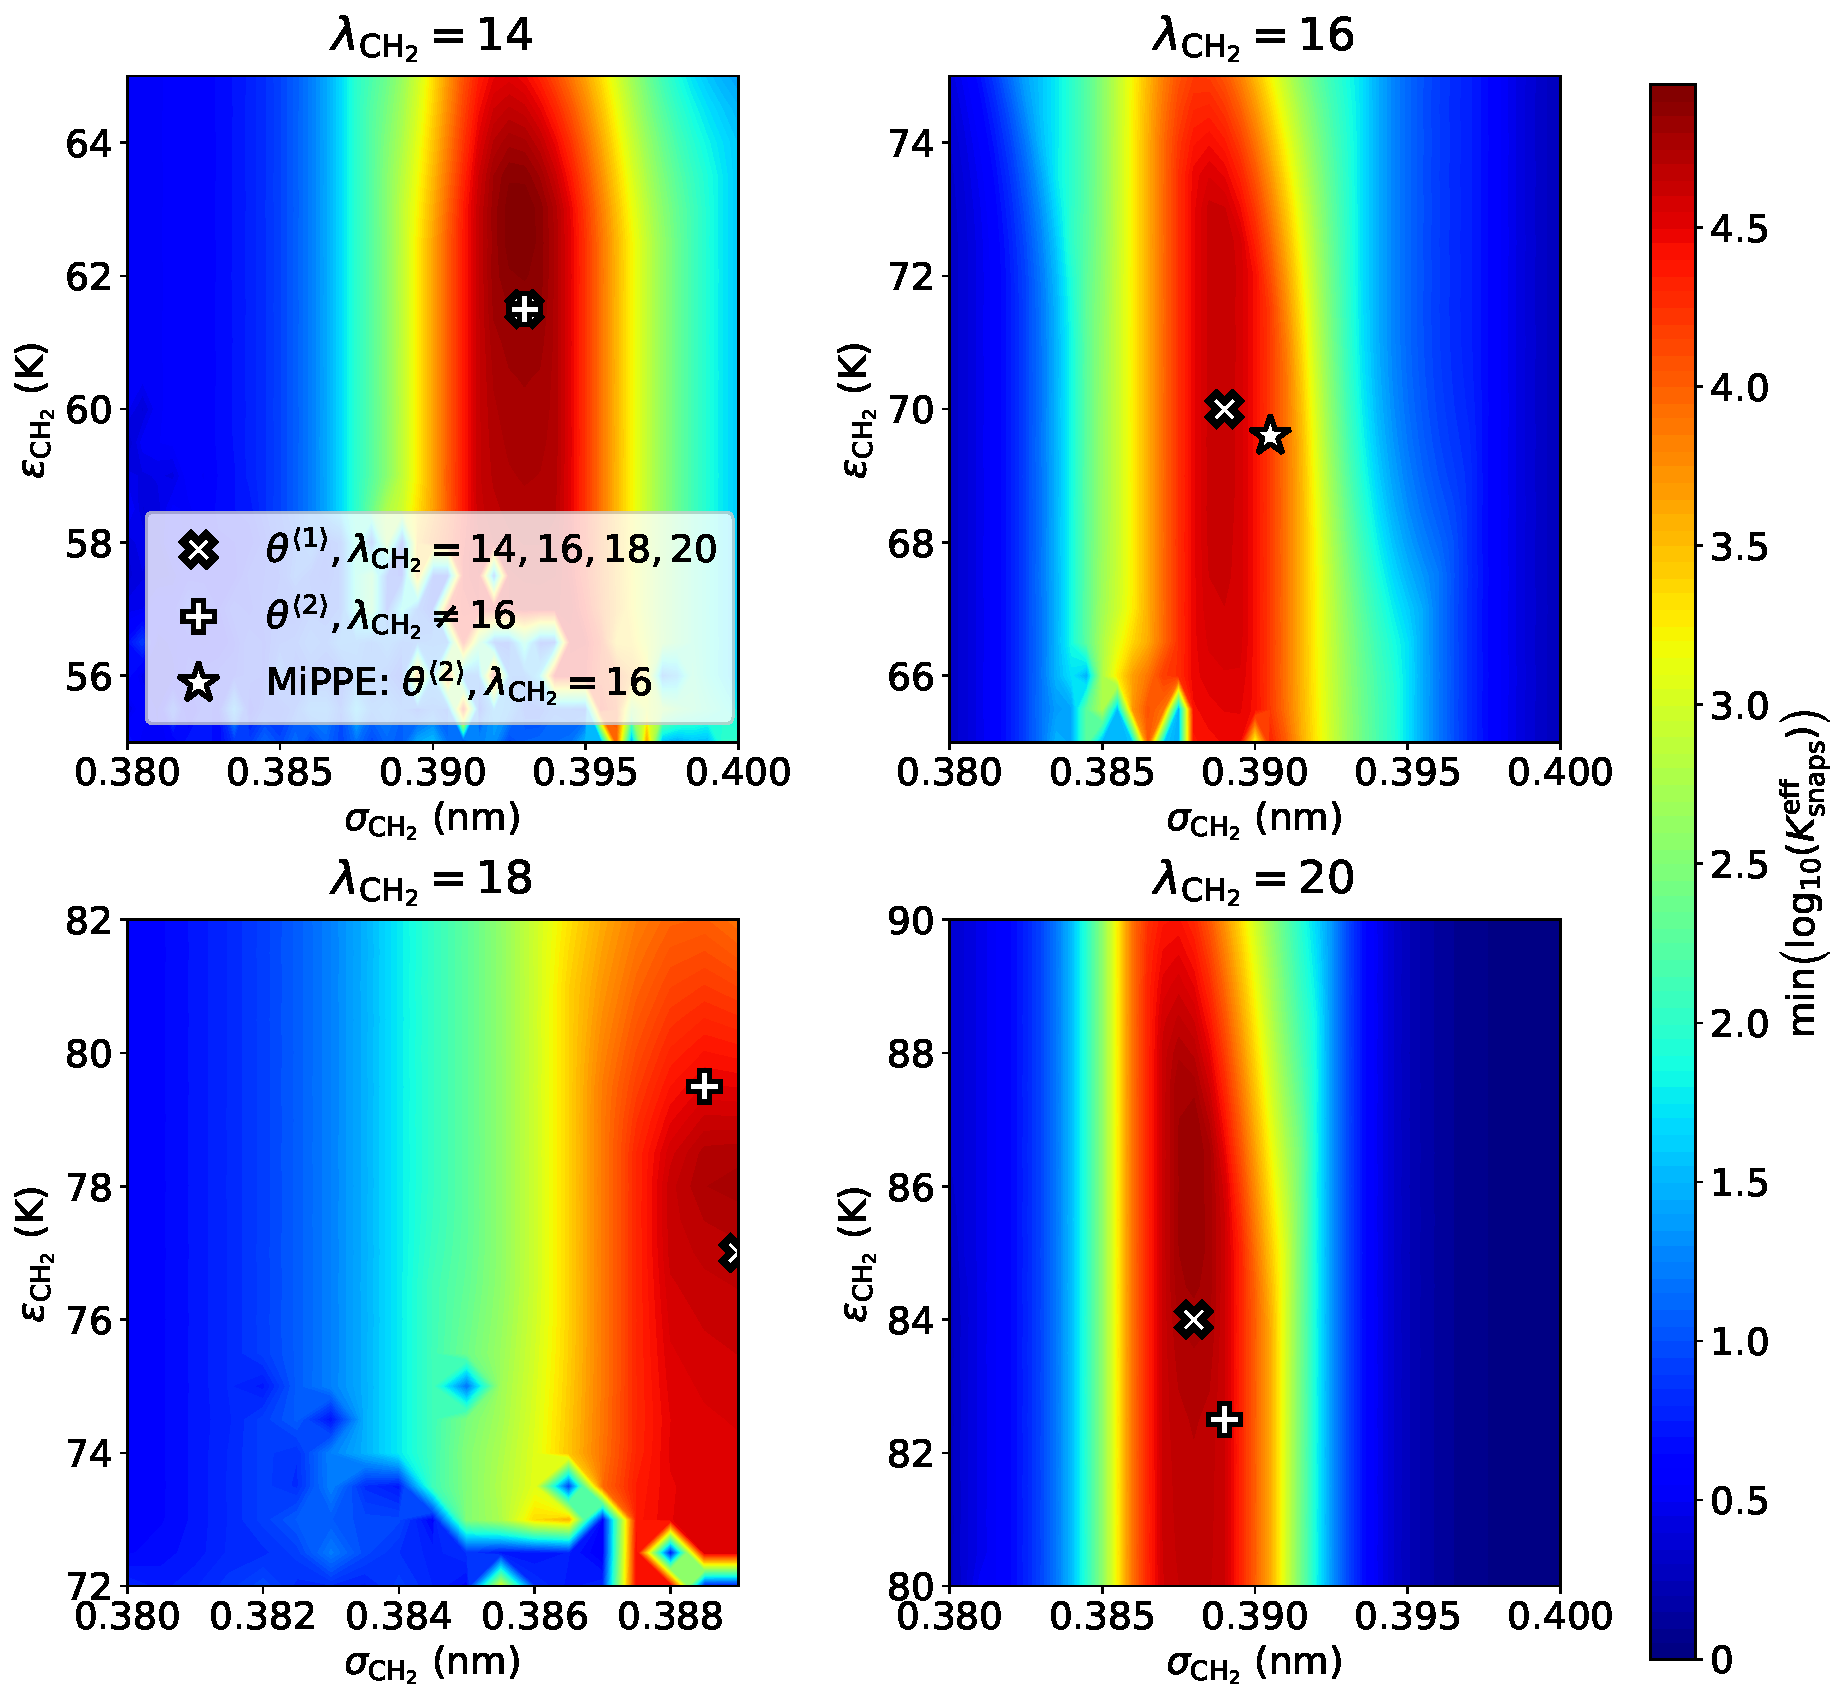
\includegraphics[width=6.4in]{CYC6_min_Neff_lam_iteration.pdf}
		\caption{Minimum number of effective snapshots $(\min(K_{\rm snaps}^{\rm eff}))$ with respect to $\epsilon_{\rm CH_2}$ and $\sigma_{\rm CH_2}$ for cyclohexane. Optimization has converged as $\min(K_{\rm snaps}^{\rm eff}) \gg 50$ for the optimal $\epsilon_{\rm CH_2}$, $\sigma_{\rm CH_2}$, $\lambda_{\rm CH_2}$ parameter set. Top-left, top-right, bottom-left, and bottom-right panels correspond $\lambda_{\rm CH_2} = 14$, $\lambda_{\rm CH_2} = 16$, $\lambda_{\rm CH_2} = 18$, and $\lambda_{\rm CH_2} = 12$, respectively. White star represents the optimal parameter set, i.e., the lowest value of $S$, for a given $\lambda_{\rm CH_2}$}
		\label{SI fig:Iterate_Neff_CYC6}
	\end{figure}

\end{document}